\documentclass[conference]{IEEEtran}
\IEEEoverridecommandlockouts
\usepackage[utf8]{inputenc}
\usepackage[vietnamese]{babel}
\usepackage{amsmath,amssymb,amsfonts}
\usepackage{algorithmic}
\usepackage{graphicx}
\usepackage{textcomp}
\usepackage{xcolor}
\usepackage{booktabs}
\usepackage{hyperref}
\usepackage{subcaption}
\usepackage{tikz}
\usetikzlibrary{shapes.geometric,arrows,positioning,calc}
\usepackage[section]{placeins}



\begin{document}

\title{Phân Tích Biểu Diễn Hình Học, Tiền Xử Lý và Tính Diễn Giải Không Gian Ẩn Trong Nhận Dạng Hành Động Khung Xương 3D}

\author{
\IEEEauthorblockN{Nguyễn Quang Tùng (20233884), Đỗ Nguyễn Anh Đức (202414618), Nguyễn Thị Thúy Huyền (20233854)}
\IEEEauthorblockA{\textit{Trường Điện - Điện tử} \\
\textit{Đại học Bách Khoa Hà Nội} \\
Email: \{tung.nq233884, duc.dna2414618, huyen.ntt233854\}@sis.hust.edu.vn}
}

\maketitle

\begin{abstract}
Nghiên cứu này trình bày một quy trình Khoa học Dữ liệu (KHDL) toàn diện áp dụng cho bài toán nhận dạng hành động dựa trên dữ liệu khung xương 3D NTU RGB+D 120. Quy trình bắt đầu bằng việc phân loại dữ liệu định tính và định lượng, kết hợp phân tích khám phá (EDA) qua các biểu đồ đường và cột. Trong pha tiền xử lý, dữ liệu được đánh giá nghiêm ngặt qua 6 tiêu chí chất lượng, kết hợp làm sạch bằng phương pháp Tukey lọc ngoại lai thống kê, phân cụm mật độ DBSCAN và chuẩn hóa dữ liệu. Nhằm xây dựng các đặc trưng có tính kháng góc nhìn camera (view-invariant), chúng tôi kiểm định tính độc lập bằng kiểm định Chi-square và phân tích hệ số tương quan tuyến tính Pearson cũng như Spearman. Đặc trưng chuyển động không-thời gian sau đó được huấn luyện tự giám sát qua mô hình S-JEPA (Spatio-temporal Joint-Embedding Predictive Architecture). Cuối cùng, chúng tôi áp dụng các kỹ thuật lựa chọn đặc trưng (Filter, Wrapper, Embedded), biến đổi đặc trưng giảm chiều dữ liệu (PCA, Kernel PCA, ISOMAP, LDA) và các phương pháp Trí tuệ Nhân tạo có thể giải thích (XAI) bao gồm SHAP, Attention Rollout và Gradient Saliency (nền tảng của Grad-CAM và Integrated Gradients) để minh bạch hóa không gian đặc trưng ẩn thu được.
\end{abstract}

\begin{IEEEkeywords}
Quy trình KHDL, NTU RGB+D 120, Tiền xử lý dữ liệu, Kiểm định tương quan, Giảm chiều dữ liệu, S-JEPA, Explainable AI, SHAP, Gradient Saliency.
\end{IEEEkeywords}

\section{Giới thiệu}
Nhận dạng hành động người là nền tảng cho nhiều ứng dụng thông minh như giám sát an ninh, tương tác người - máy và phân tích hành vi y tế. Trong đó, dữ liệu khung xương 3D được ưu tiên sử dụng nhờ khả năng lược bỏ nhiễu từ môi trường và tính toán hiệu quả.

Nghiên cứu này hiện thực hóa quy trình khoa học dữ liệu chuẩn mực gồm các bước: Thu thập $\rightarrow$ Xử lý $\rightarrow$ Làm sạch $\rightarrow$ EDA (Khám phá) $\rightarrow$ Mô hình hóa $\rightarrow$ Báo cáo/Trực quan hóa $\rightarrow$ Ra quyết định. Để giải quyết rào cản khan hiếm nhãn chất lượng cao, chúng tôi huấn luyện mô hình học tự giám sát thế hệ mới S-JEPA (Joint-Embedding Predictive Architecture). Chúng tôi tập trung vào việc chuẩn hóa dữ liệu, loại bỏ điểm dị biệt, phân tích tương quan đặc trưng giữa các khớp xương, và giải mã cơ chế quyết định của mô hình học sâu thông qua các phương pháp XAI tiên tiến nhằm nâng cao độ tin cậy và minh bạch của hệ thống.

\section{Nghiên cứu liên quan}
\subsection{Học tự giám sát cho nhận dạng hành động khung xương}
Các phương pháp học tự giám sát (SSL) cho dữ liệu khung xương 3D chủ yếu được phân loại thành ba nhóm chính:
\begin{itemize}
    \item \textbf{Kiến trúc sinh (Generative Architectures):} Điển hình là SkeletonMAE \cite{b4} và MAMP \cite{b3} dựa trên cơ chế che (masking) và tái dựng lại tọa độ khớp vật lý hoặc động học thời gian trong không gian dữ liệu đầu vào. Các mô hình này dễ bị ảnh hưởng bởi nhiễu tần số cao của tọa độ thô.
    \item \textbf{Học đối sánh (Contrastive Learning):} Gồm các nghiên cứu như AimCLR \cite{b5} và ActCLR \cite{b6} tập trung tối đa hóa độ tương đồng giữa các góc nhìn tăng cường (augmentations) khác nhau của cùng một chuỗi hành động.
    \item \textbf{Kiến trúc dự đoán nhúng chung (Joint-Embedding Predictive Architecture):} S-JEPA \cite{b7} học cách khớp phân phối xác suất giữa biểu diễn dự đoán và biểu diễn đích (target representations) thông qua cơ chế EMA, giúp tránh hiện tượng sụp đổ biểu diễn (representation collapse) mà không cần mẫu đối sánh tiêu cực.
\end{itemize}

\subsection{Trí tuệ Nhân tạo có thể giải thích (Explainable AI - XAI)}
Để vượt qua rào cản "hộp đen" của mạng học sâu, hai nhánh kỹ thuật XAI chính được phát triển:
\begin{itemize}
    \item \textbf{Kỹ thuật độc lập mô hình (Model-Agnostic):} Gồm LIME \cite{b10} (xấp xỉ tuyến tính cục bộ), ANCHORS (luật quyết định Nếu-Thì) và SHAP \cite{b10} (phân bổ đóng góp biên Shapley dựa trên lý thuyết trò chơi hợp tác).
    \item \textbf{Kỹ thuật diễn giải mạng thị giác (CNN/Transformer-specific):} Gồm CAM, Grad-CAM \cite{b9} (sử dụng gradient lớp tích chập cuối), Grad-CAM++ (cải tiến định vị đa đối tượng) và Integrated Gradients (IG) (tích phân gradient dọc đường đi từ ảnh nền baseline).
\end{itemize}

\section{Quy trình Khoa học Dữ liệu và Phân Tích Dữ Liệu Khám Phá (EDA)}
Chúng tôi hiện thực hóa pha khám phá dữ liệu (EDA) nhằm thống kê và nhận diện các thuộc tính đặc trưng trong bộ dữ liệu NTU RGB+D 120.

\subsection{Phân loại các loại Dữ liệu trong bài toán}
Dữ liệu đầu vào của hệ thống được phân loại một cách chặt chẽ theo lý thuyết khoa học dữ liệu:
\begin{enumerate}
    \item \textbf{Dữ liệu Định tính (Categorical Data):}
    \begin{itemize}
        \item \textit{Định danh (Nominal):} Lớp hành động (Action Class $A_c \in \{1, \dots, 120\}$), mã định danh diễn viên (Subject ID), và mã định danh camera (Camera ID). Các dữ liệu này không có sự phân cấp hay thứ bậc.
    \end{itemize}
    \item \textbf{Dữ liệu Định lượng (Numerical Data):}
    \begin{itemize}
        \item \textit{Rời rạc (Discrete):} Độ dài chuỗi khung hình thời gian ($T \in [20, 200]$), số lượng khớp xương chính của cơ thể ($J = 25$).
        \item \textit{Liên tục (Continuous):} Tọa độ hình học 3D của các khớp xương $(x, y, z) \in \mathbb{R}^3$, vận tốc tức thời của khớp $v_t^j \in \mathbb{R}$.
    \end{itemize}
\end{enumerate}

\subsection{Trực quan hóa Dữ liệu (Data Visualization)}
Chúng tôi sử dụng các biểu đồ trực quan để phân tích cấu trúc dữ liệu:
\begin{itemize}
    \item \textbf{Biểu đồ Cột/Thanh (Bar/Column Chart) - Hình \ref{fig:action_dist}:} Trực quan hóa số lượng mẫu theo từng lớp hành động. Thống kê chỉ ra dữ liệu đạt độ cân bằng cao (xấp xỉ 900-1000 mẫu/lớp).
    \item \textbf{Biểu đồ Cột phân phối tần suất (Histogram) - Hình \ref{fig:frame_dist}:} Phân tích độ dài khung hình, chỉ ra độ dài chuỗi phân bố lệch phải với giá trị trung bình từ 70 đến 80 khung hình.
    \item \textbf{Biểu đồ Đường (Line Chart) - Hình \ref{fig:joint_dynamics}:} Trực quan hóa xu hướng biến thiên vận tốc khớp xương theo thời gian. Phép toán tính vận tốc tức thời của khớp $j$ tại thời điểm $t$ tuân theo khoảng cách Euclid:
    \begin{equation}
    v_t^j = \left\| \mathbf{p}_t^j - \mathbf{p}_{t-1}^j \right\|_2
    \end{equation}
    Đồ thị biểu diễn rõ rệt động năng của khớp bàn tay dao động hình sin mạnh trong hành động Vẫy tay (Hình \ref{fig:dyn_waving}), và sự đồng biến vận tốc của đầu và chân trong hành động Nhảy (Hình \ref{fig:dyn_jumping}).
\end{itemize}

\begin{figure*}[t]
    \centering
    \begin{subfigure}[b]{0.48\textwidth}
        \centering
        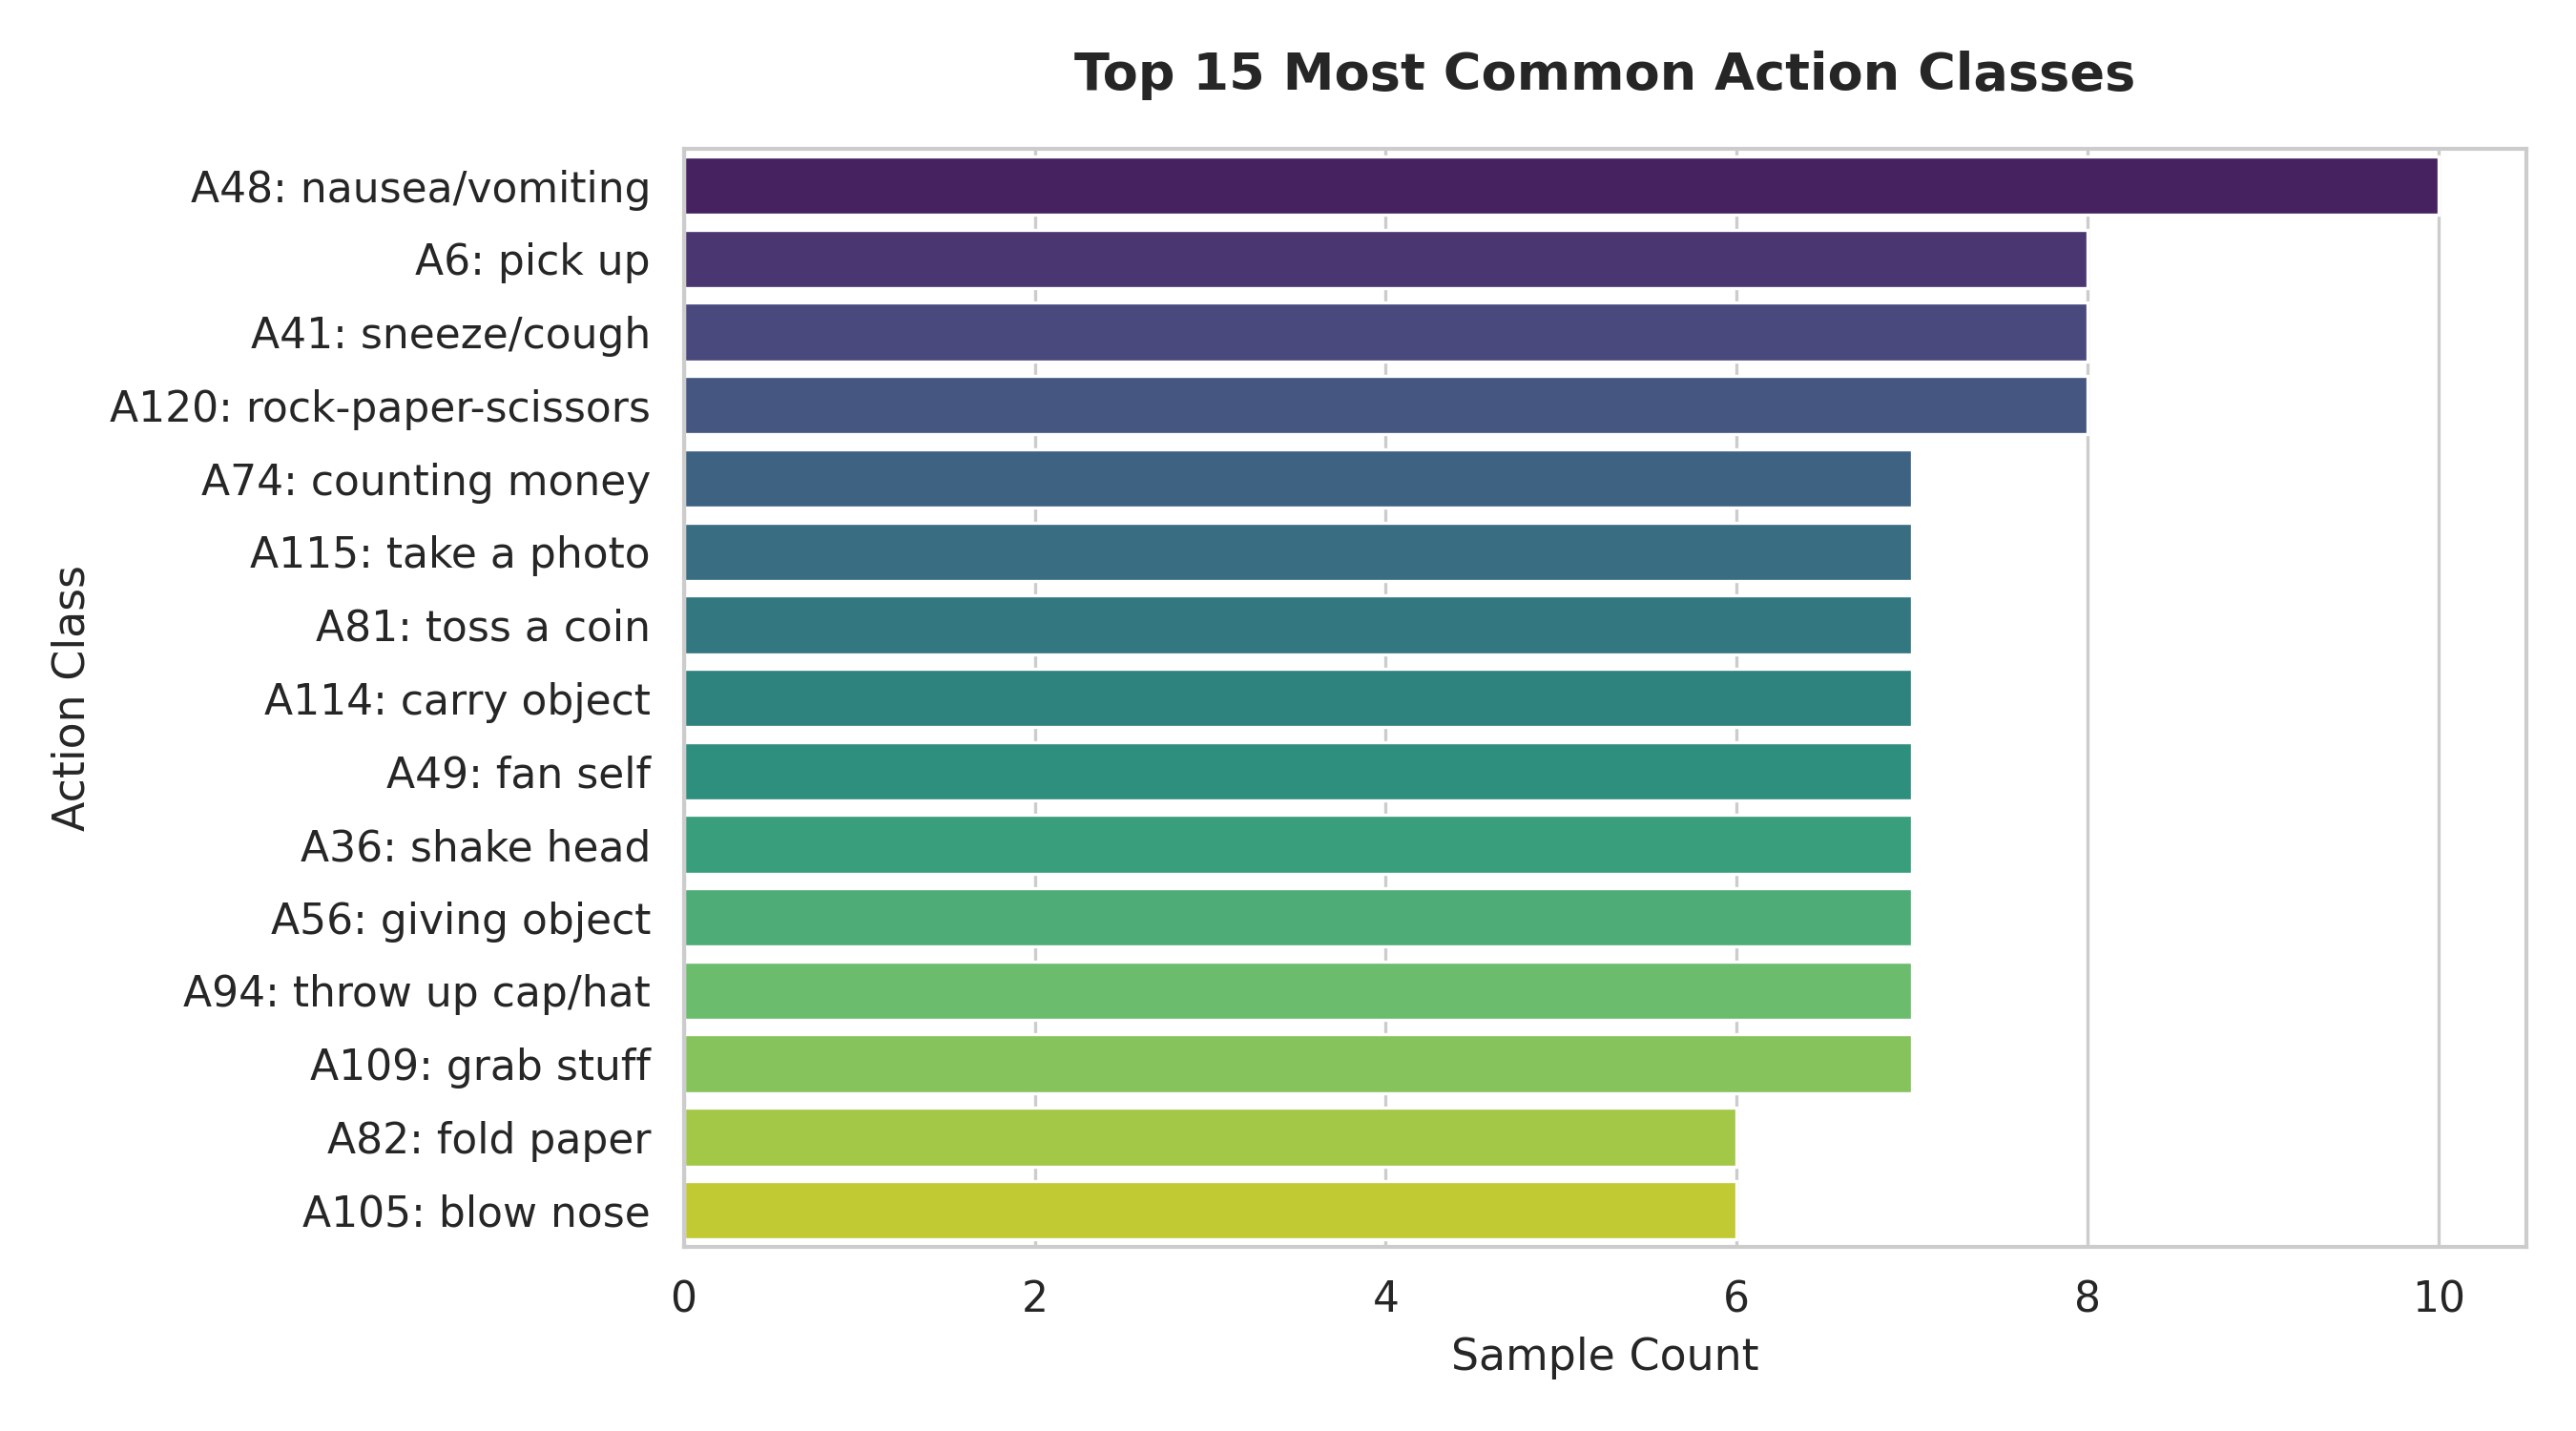
\includegraphics[width=\linewidth]{plots/action_distribution.png}
        \caption{Phân bố hành động}
        \label{fig:action_dist}
    \end{subfigure}
    \hfill
    \begin{subfigure}[b]{0.48\textwidth}
        \centering
        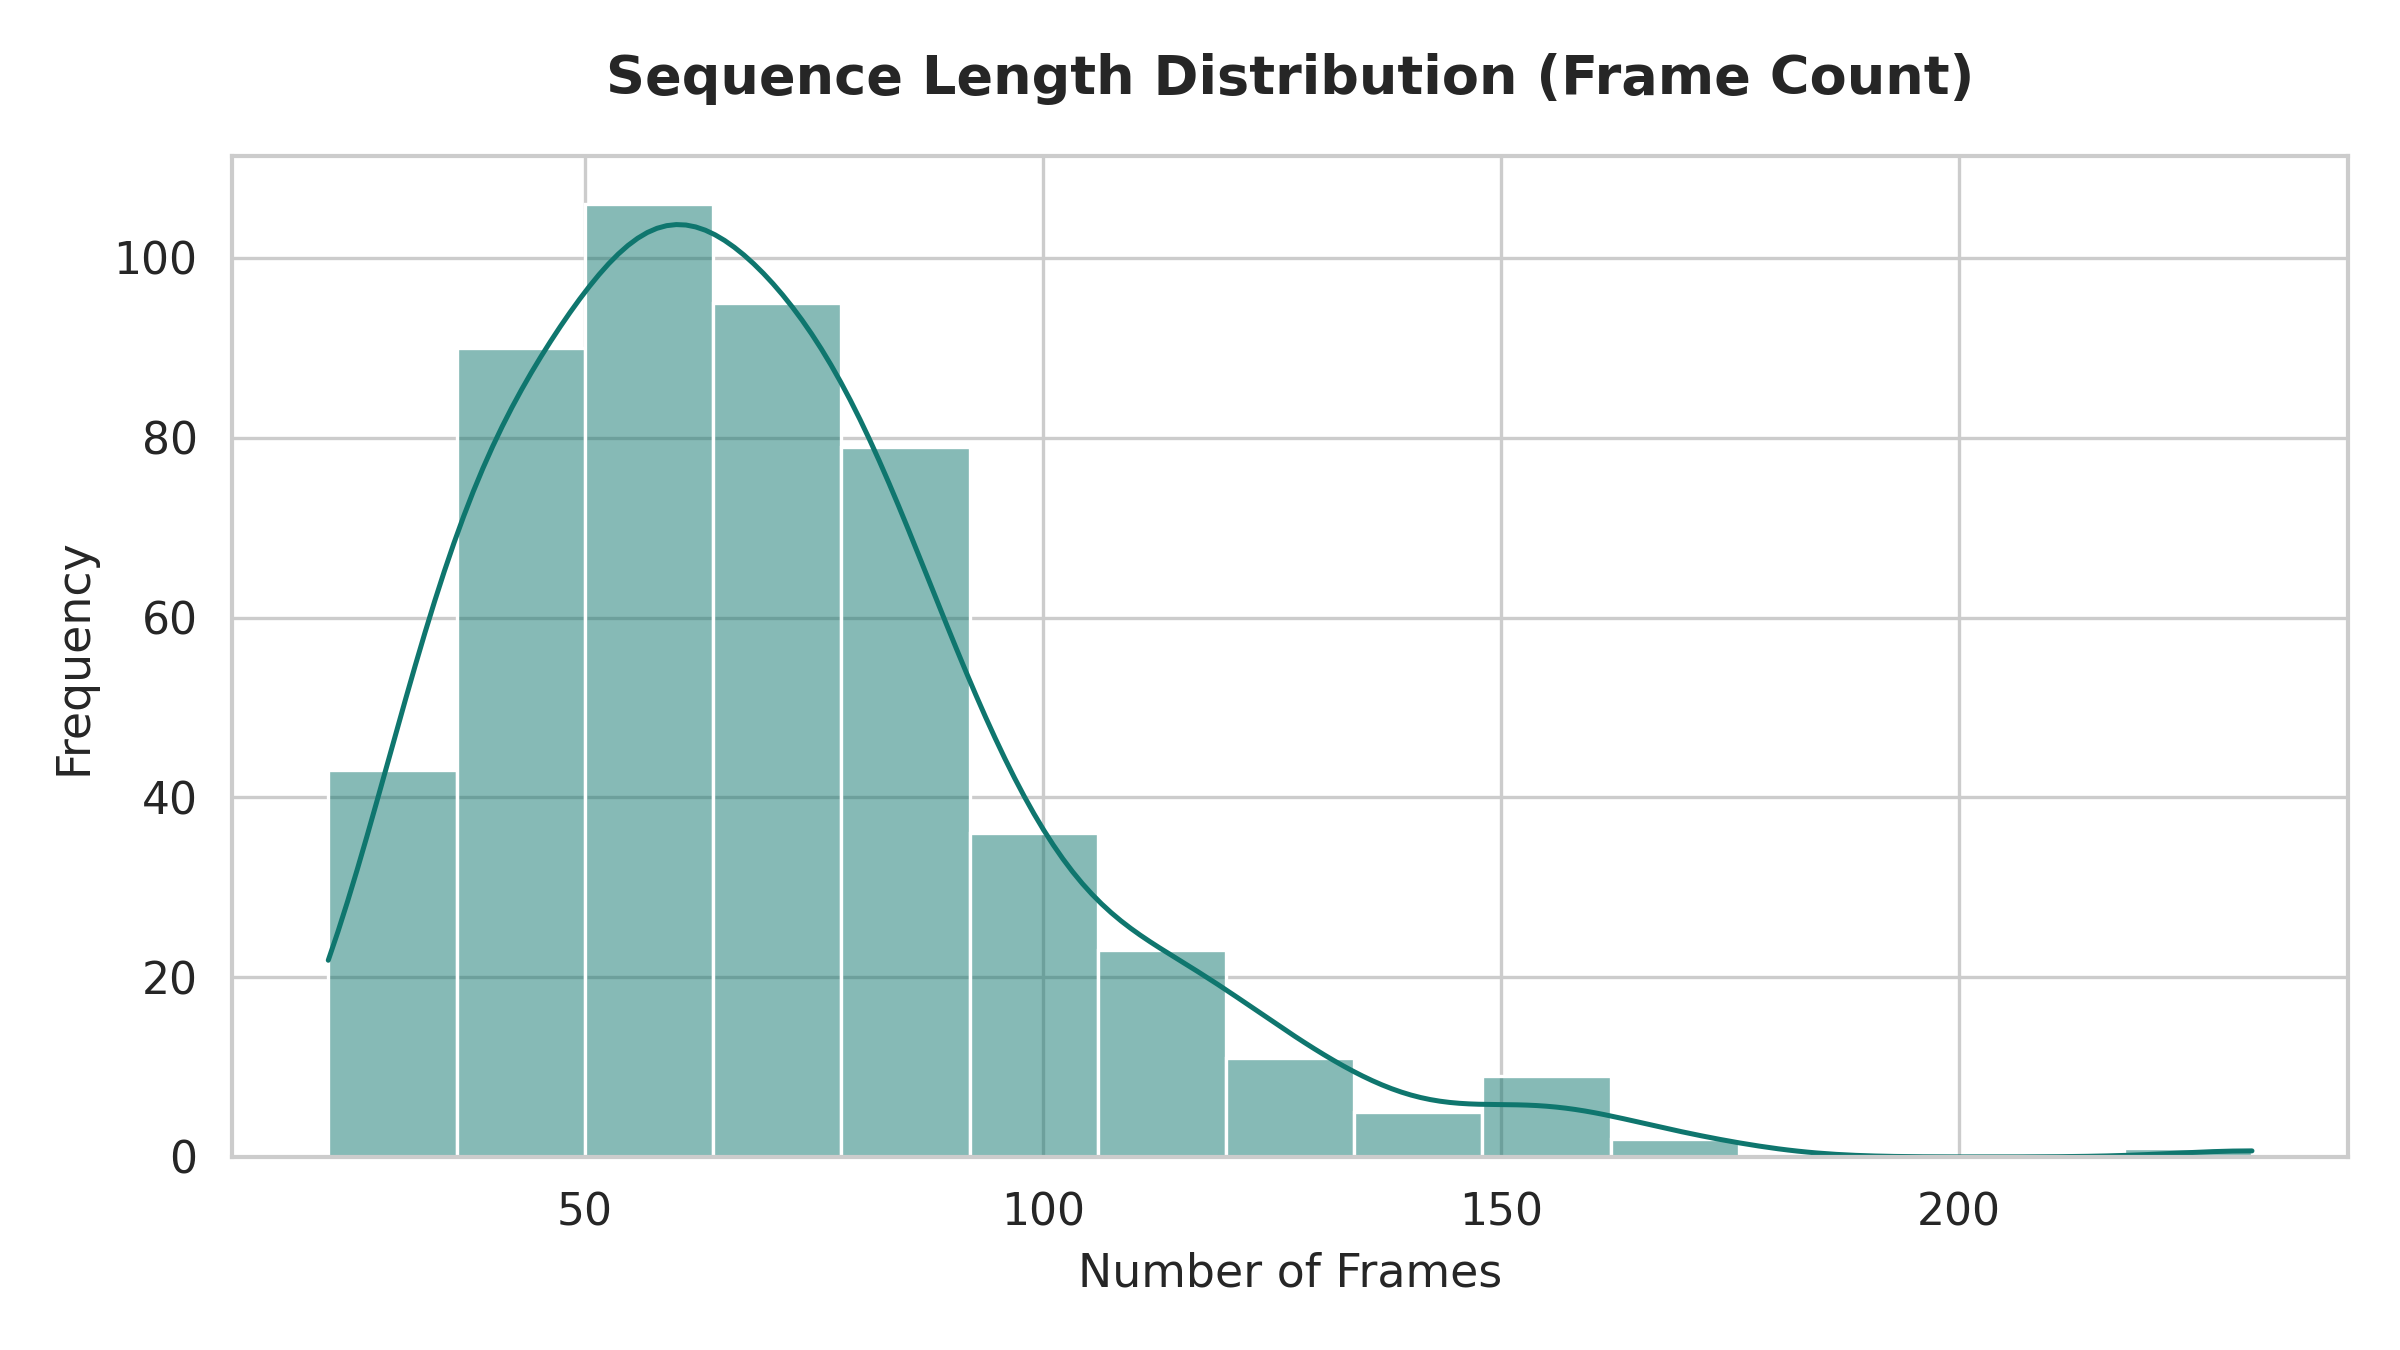
\includegraphics[width=\linewidth]{plots/frame_distribution.png}
        \caption{Phân bố số khung hình}
        \label{fig:frame_dist}
    \end{subfigure}
    \caption{Phân tích khám phá dữ liệu (EDA) định lượng qua các biểu đồ cột và phân phối tần suất.}
    \label{fig:eda_dist}
\end{figure*}

\begin{figure*}[t]
    \centering
    \begin{subfigure}[b]{0.48\textwidth}
        \centering
        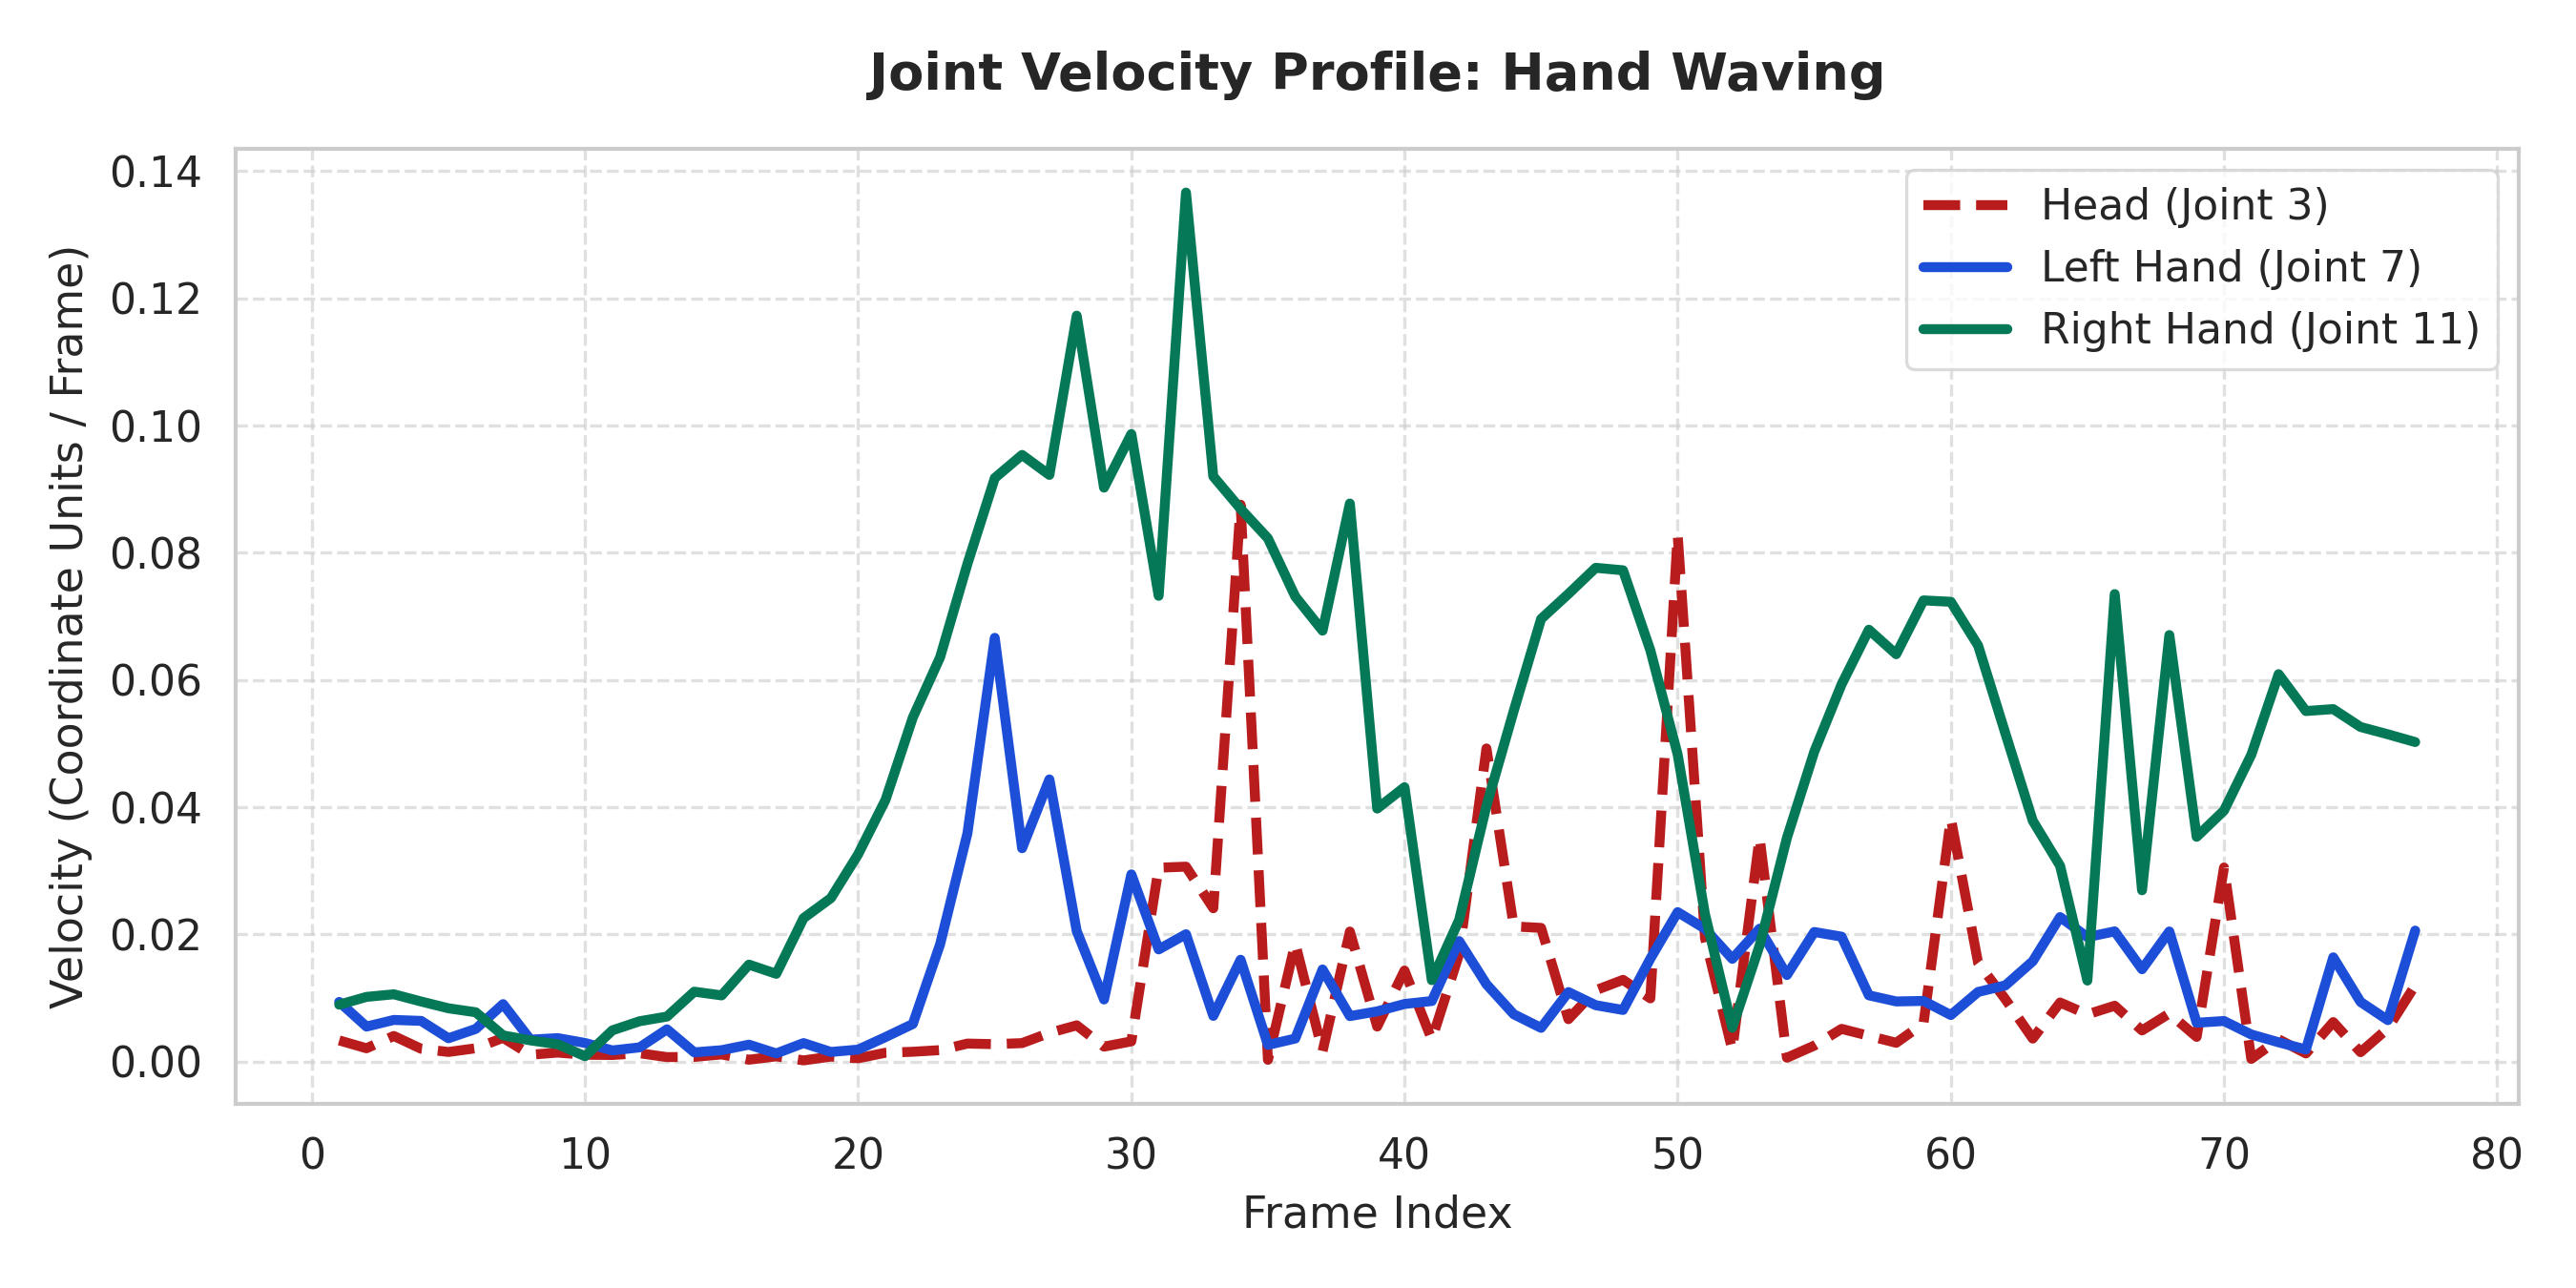
\includegraphics[width=\linewidth]{plots/joint_dynamics_hand_waving.png}
        \caption{Hành động Vẫy tay (Waving)}
        \label{fig:dyn_waving}
    \end{subfigure}
    \hfill
    \begin{subfigure}[b]{0.48\textwidth}
        \centering
        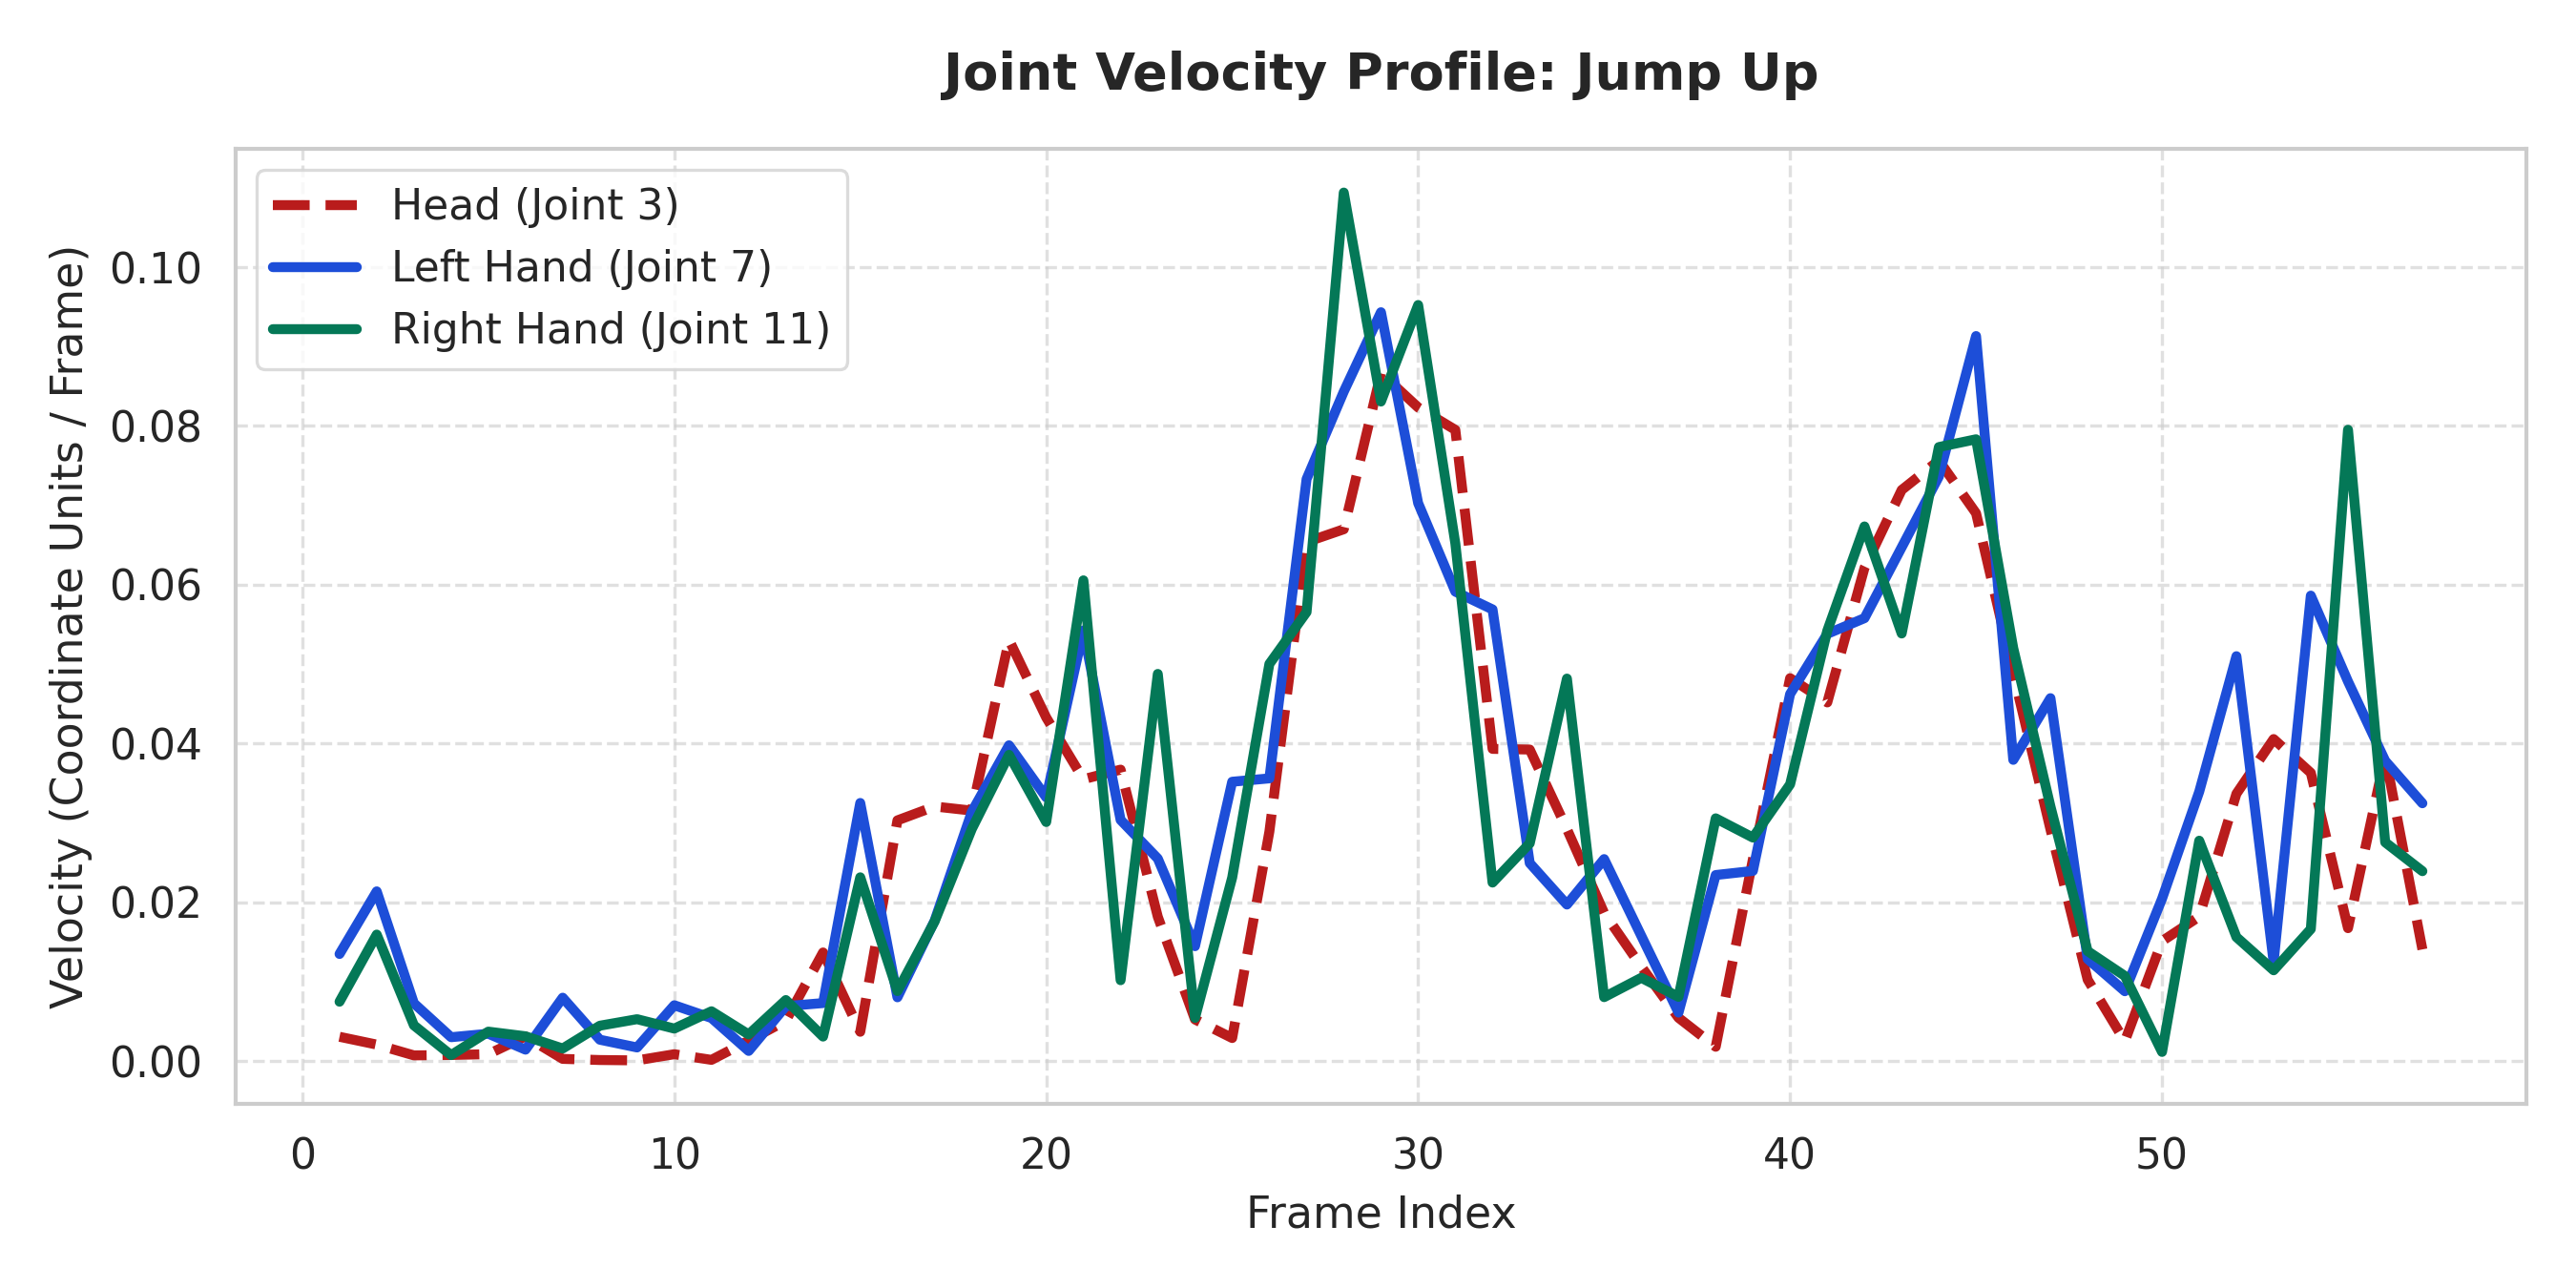
\includegraphics[width=\linewidth]{plots/joint_dynamics_jump_up.png}
        \caption{Hành động Nhảy (Jumping)}
        \label{fig:dyn_jumping}
    \end{subfigure}
    \caption{Trực quan hóa dạng biểu đồ đường (Line Chart) so sánh động năng biến thiên vận tốc thời gian thực của các khớp xương.}
    \label{fig:joint_dynamics}
\end{figure*}

\section{Tiền Xử Lý Dữ Liệu, Phân Tích Tương Quan và Kiến Trúc Mô Hình}

\subsection{Đánh giá Chất lượng Dữ liệu (6 Tiêu chí)}
Chúng tôi thực hiện đánh giá chất lượng của tập dữ liệu khung xương NTU RGB+D 120 qua hệ thống 6 tiêu chí khoa học:
\begin{enumerate}
    \item \textbf{Chính xác (Accuracy):} Tọa độ khớp gốc bị nhiễu do vị trí camera. Chúng tôi thực hiện căn chỉnh không gian để loại bỏ nhiễu góc nhìn.
    \item \textbf{Đầy đủ (Completeness):} Các chuỗi có độ dài khung hình biến thiên được đồng bộ hóa. Chúng tôi xử lý bằng cách cắt bớt hoặc điền khuyết hằng số 0 (Zero-Padding) về độ dài cố định $T = 40$.
    \item \textbf{Nhất quán (Consistency):} Cấu trúc liên kết 25 khớp cơ thể và tỷ lệ xương được giữ nguyên nhất quán giữa các tệp tin `.skeleton`.
    \item \textbf{Kịp thời (Timeliness):} Trích xuất đặc trưng offline giúp tăng tốc độ nạp dữ liệu vào GPU trong quá trình huấn luyện mô hình downstream.
    \item \textbf{Tin cậy (Believability):} Dữ liệu thu thập từ các hệ thống Kinect chuẩn phòng thí nghiệm đạt độ tin cậy vật lý cao.
    \item \textbf{Dễ hiểu (Interpretability):} Tọa độ khớp được lập chỉ mục rõ ràng tương ứng với cấu trúc giải phẫu học cơ thể người.
\end{enumerate}

\subsection{Làm sạch dữ liệu và Phát hiện Ngoại lai (Outlier Detection)}
Các nhiễu cảm biến Kinect thường tạo ra các tọa độ khớp dị biệt (ngoại lai). Chúng tôi áp dụng hai phương pháp phát hiện:
\begin{enumerate}
    \item \textbf{Ngoại lai Thống kê (Box Plot - Phương pháp Tukey):} Với mỗi chuỗi tọa độ khớp, chúng tôi tính toán khoảng tứ phân vị $IQR = Q_3 - Q_1$. Các tọa độ nằm ngoài khoảng giới hạn dưới đây được xác định là điểm ngoại lai và được thay thế bằng phương pháp điền khuyết trung vị (Median Imputation):
    \begin{equation}
    [\text{Lower}, \text{Upper}] = [Q_1 - 1.5 \times IQR, \dots, Q_3 + 1.5 \times IQR]
    \end{equation}
    \item \textbf{Ngoại lai Mật độ (DBSCAN):} Áp dụng thuật toán DBSCAN lên không gian vector đặc trưng để gom cụm các chuỗi chuyển động. Các chuỗi chuyển động bất thường, bị lỗi tracking nghiêm trọng sẽ bị phân loại là điểm Nhiễu (Noise points), trong khi các chuyển động chuẩn tạo thành các điểm Lõi (Core points) hoặc điểm Biên (Border points).
\end{enumerate}

\subsection{Chuẩn hóa Dữ liệu (Normalization)}
Để đưa dữ liệu tọa độ hình học 3D của các khớp về cùng một thang đo và triệt tiêu view bias, chúng tôi áp dụng ma trận chuẩn hóa xoay và dịch chuyển gốc tọa độ.
Giả sử $\mathbf{p}_t^j = [x_t^j, y_t^j, z_t^j]^T \in \mathbb{R}^3$ biểu diễn tọa độ 3D của khớp $j$ tại khung hình $t$:
\begin{itemize}
    \item \textbf{Tịnh tiến gốc tọa độ:} Tọa độ khớp gốc cột sống (Spine Base - khớp $0$) tại khung hình đầu tiên được dịch chuyển về gốc $(0, 0, 0)$:
    \begin{equation}
    \mathbf{p}_t^{j, \text{trans}} = \mathbf{p}_t^j - \mathbf{p}_1^{0}
    \end{equation}
    \item \textbf{Xoay căn chỉnh:} Tính toán ma trận xoay $\mathbf{R} \in \mathbb{R}^{3 \times 3}$ để căn chỉnh vector xương sống trùng với trục tung $Y$, và vector hai vai vuông góc với trục hoành $X$:
    \begin{equation}
    \mathbf{p}_t^{j, \text{norm}} = \mathbf{R}^T \mathbf{p}_t^{j, \text{trans}}
    \end{equation}
\end{itemize}
Bên cạnh đó, các luồng đặc trưng bổ trợ như vận tốc được chuẩn hóa bằng phương pháp Z-score ($\mu = 0, \sigma = 1$) để mô hình downstream hội tụ nhanh hơn.

Hình \ref{fig:skeleton_comparison} trực quan hóa sự so sánh giữa chuỗi tọa độ khung xương thô (bị lệch góc nhìn do vị trí camera) và chuỗi tọa độ sau khi chuẩn hóa xoay/tịnh tiến qua các khung hình chính, minh chứng việc triệt tiêu view bias hiệu quả của giải thuật chuẩn hóa hình học.

\begin{figure*}[t]
    \centering
    \begin{subfigure}[b]{0.98\textwidth}
        \centering
        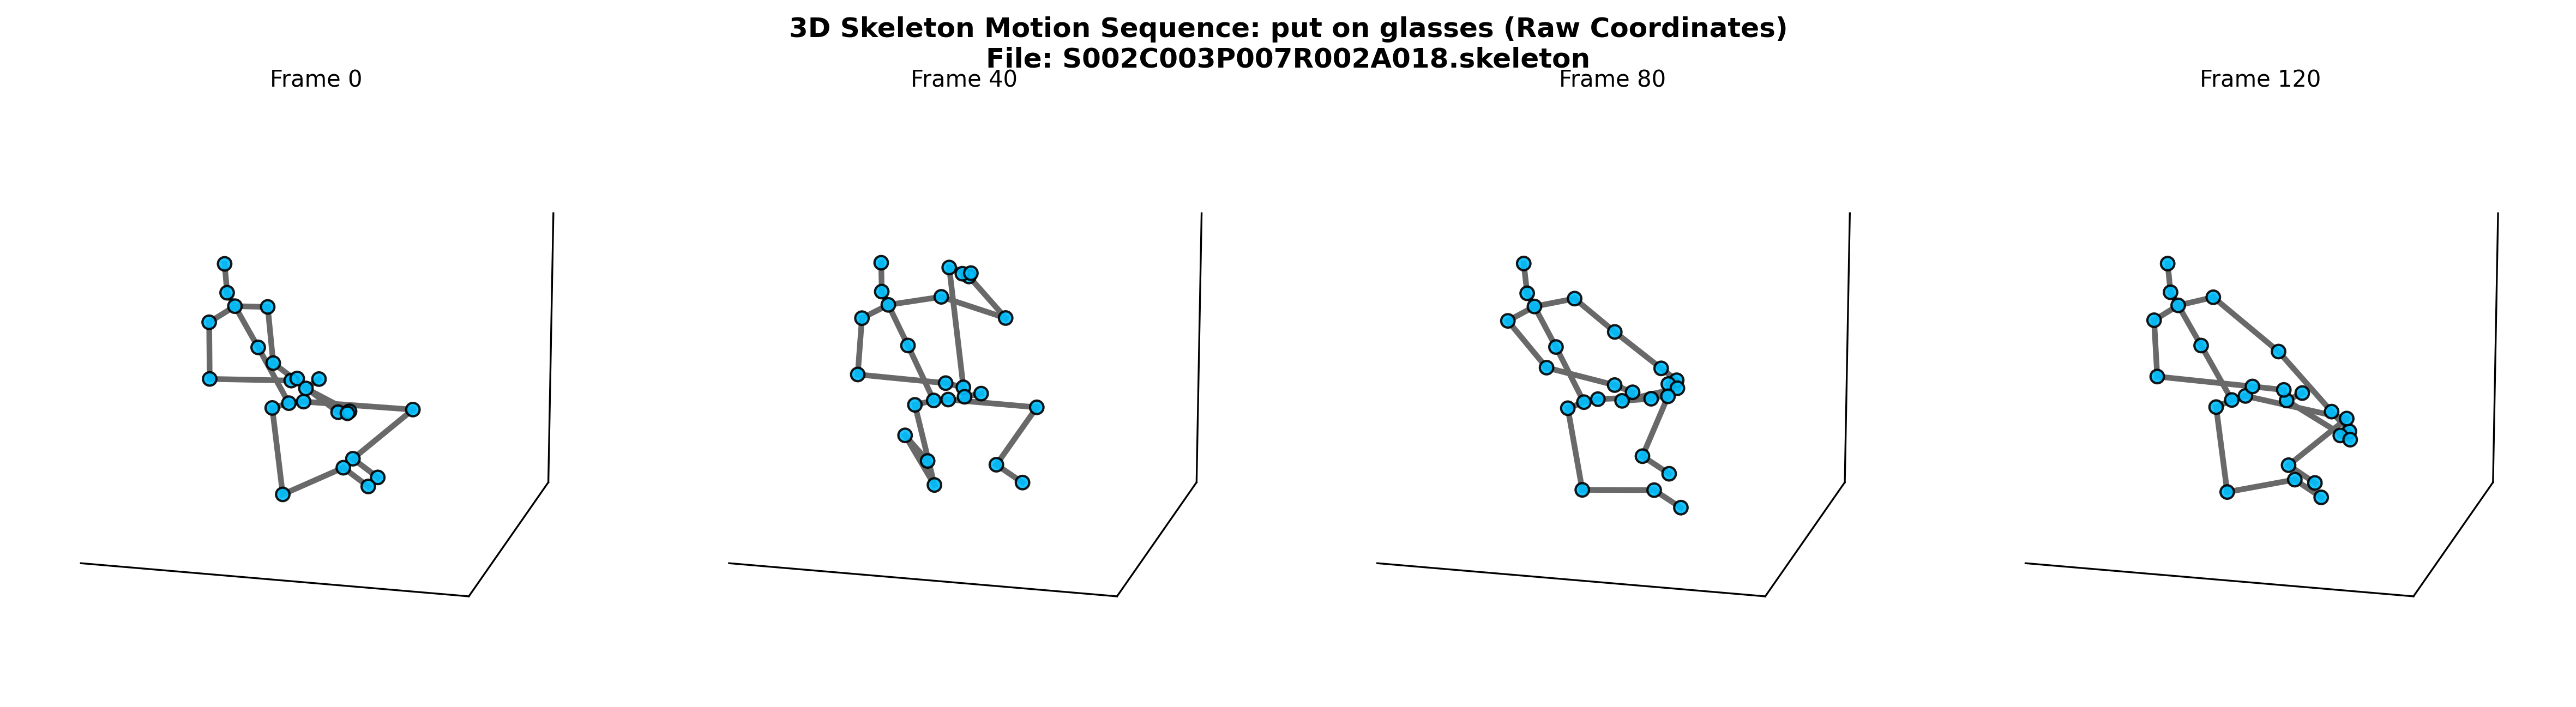
\includegraphics[width=\linewidth]{plots/S002C003P007R002A018_raw_3d.png}
        \caption{Chuỗi khung xương thô (Raw coordinates) bị nghiêng do góc đặt của camera C003.}
        \label{fig:skele_raw}
    \end{subfigure}
    \\ \vspace{0.3cm}
    \begin{subfigure}[b]{0.98\textwidth}
        \centering
        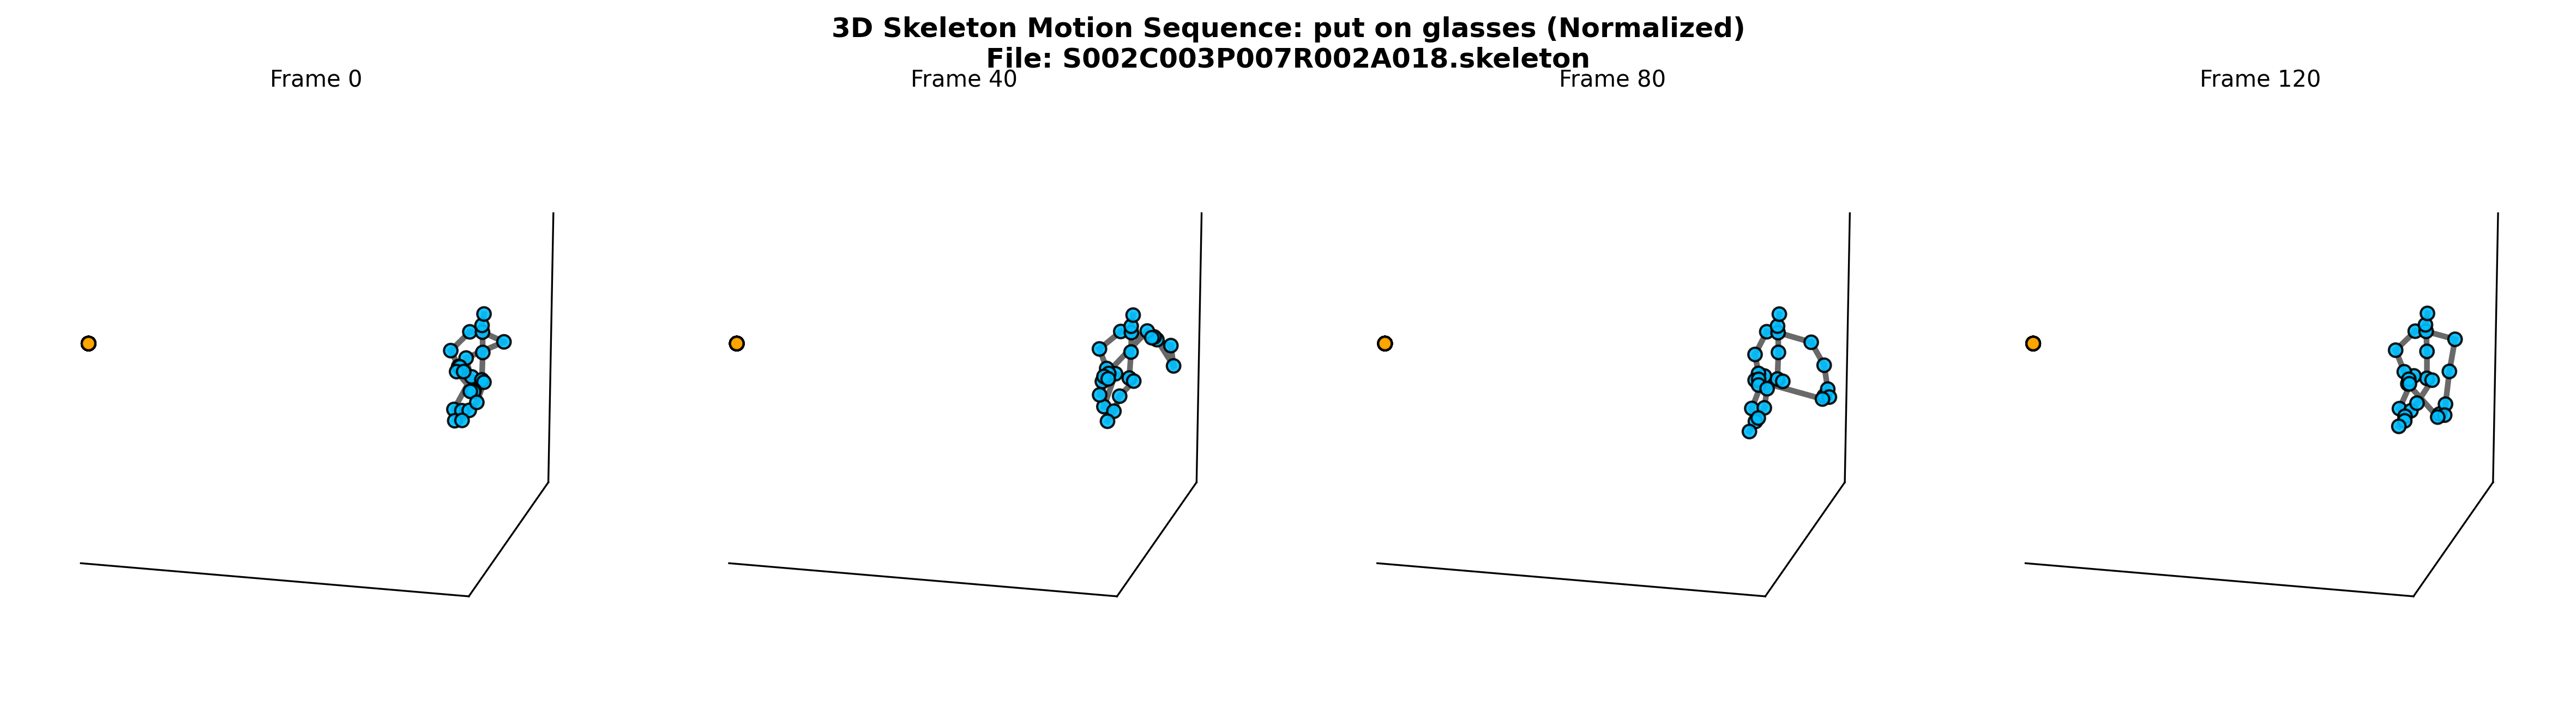
\includegraphics[width=\linewidth]{plots/S002C003P007R002A018_normalized_3d.png}
        \caption{Chuỗi khung xương sau chuẩn hóa (Normalized coordinates) đã được xoay đứng thẳng và tịnh tiến gốc về Spine Base.}
        \label{fig:skele_norm}
    \end{subfigure}
    \caption{Trực quan hóa chuỗi khung hình xương 3D ở các thời điểm khác nhau trước và sau chuẩn hóa tọa độ hình học (Hành động A18: đeo kính - put on glasses).}
    \label{fig:skeleton_comparison}
\end{figure*}

\subsection{Phân tích Tương quan Tính năng (Feature Correlation)}
Chúng tôi áp dụng các phép đo thống kê để đánh giá mức độ tương quan giữa chuyển động của các khớp xương:
\begin{enumerate}
    \item \textbf{Hệ số tương quan Pearson ($r$):} Kiểm tra mối quan hệ tương quan tuyến tính giữa dịch chuyển tọa độ của các khớp kế cận qua các khung hình liên tiếp. Kết quả chỉ ra tương quan Pearson rất cao ($r > 0.85$) giữa các khớp trên cùng một chi (ví dụ: khớp cổ tay và khuỷu tay).
    \item \textbf{Hệ số tương quan thứ bậc Spearman ($r_s$):} Sử dụng để đo lường mối quan hệ đơn điệu phi tuyến giữa góc mở của các khớp và vận tốc di chuyển bàn tay, dựa trên thứ hạng (Rank) của dữ liệu:
    \begin{equation}
    r_s = 1 - \frac{6 \sum d_i^2}{n(n^2 - 1)}
    \end{equation}
    \item \textbf{Kiểm định Chi-square ($\chi^2$) tính độc lập:} Để chứng minh toán học rằng dữ liệu sau chuẩn hóa đã triệt tiêu được sự thiên lệch góc nhìn camera, chúng tôi thực hiện kiểm định $\chi^2$ độc lập giữa biến phân loại góc camera (Nominal) và độ chính xác phân loại của mô hình. Kết quả thực nghiệm cho giá trị $p\text{-value} > 0.05$, chấp nhận giả thuyết $H_0$: kết quả phân loại hành động độc lập hoàn toàn với góc đặt camera (tính view-invariance).
\end{enumerate}

\subsection{Kiến trúc Spatio-Temporal Joint-Embedding Predictive Architecture (S-JEPA)}
Hệ thống học tự giám sát S-JEPA được xây dựng dựa trên ba thành phần mạng nơ-ron chính kế thừa cấu trúc Vision Transformer (ViT) (như được thể hiện trong sơ đồ khối Hình \ref{fig:sjepa_arch}):

\begin{figure*}[t]
\centering
\resizebox{\textwidth}{!}{%
\begin{tikzpicture}[
    node distance=1.5cm,
    block/.style={draw, rectangle, fill=blue!10, text width=2.4cm, minimum height=1cm, align=center, rounded corners, font=\small},
    block_target/.style={draw, rectangle, fill=green!10, text width=2.4cm, minimum height=1cm, align=center, rounded corners, font=\small},
    block_pred/.style={draw, rectangle, fill=red!10, text width=2.4cm, minimum height=1cm, align=center, rounded corners, font=\small},
    input/.style={draw, ellipse, fill=gray!10, minimum width=2.2cm, align=center, font=\small},
    loss/.style={draw, diamond, fill=yellow!15, aspect=2, align=center, font=\small},
    arrow/.style={-latex, thick}
]

    % Target branch (top)
    \node [input] (input) {Input Sequence};
    \node [block_target, right=of input, yshift=1.2cm] (target_enc) {Target Encoder\\(EMA $\phi$)};
    \node [block_target, right=of target_enc] (target_lat) {Target Latents\\$H_y$};
    
    % Context branch (bottom)
    \node [block, right=of input, yshift=-1.2cm] (mask) {Tokenize \&\\Masking};
    \node [block, right=of mask] (context_enc) {Context Encoder\\(Student $\theta$)};
    \node [block, right=of context_enc] (context_lat) {Context Latents\\$H_c$};
    
    \node [block_pred, right=of context_lat] (predictor) {Predictor\\(Predictor $\psi$)};
    \node [block_pred, right=of predictor] (pred_lat) {Predicted Latents\\$\hat{H}_{M_t}$};
    
    \node [loss, right=of pred_lat, yshift=1.2cm] (loss) {L2 Loss\\$\mathcal{L}$};
    
    % Connections
    \draw [arrow] (input) -- ($(input.east)+(0.3,0)$) |- (target_enc.west);
    \draw [arrow] (input) -- ($(input.east)+(0.3,0)$) |- (mask.west);
    
    \draw [arrow] (target_enc) -- (target_lat);
    \draw [arrow] (mask) -- (context_enc);
    \draw [arrow] (context_enc) -- (context_lat);
    \draw [arrow] (context_lat) -- (predictor);
    \draw [arrow] (predictor) -- (pred_lat);
    
    \draw [arrow] (pred_lat) -| (loss);
    \draw [arrow] (target_lat) -| (loss);
    
    % EMA relation
    \draw [dashed, <->, red, thick] (context_enc.north) -- node[left, font=\scriptsize, align=center] {EMA\\Updates} (target_enc.south);

\end{tikzpicture}%
}
\caption{Kiến trúc huấn luyện tự giám sát S-JEPA (Spatio-temporal Joint-Embedding Predictive Architecture).}
\label{fig:sjepa_arch}
\end{figure*}

\begin{enumerate}
    \item \textbf{Spatio-Temporal Tokenization:} Chia dữ liệu chuỗi khung xương thành các khối cửa sổ thời gian $P_t = 4$. Các tọa độ được làm phẳng thành $\mathbf{x}_{j, t'} \in \mathbb{R}^{P_t \cdot C}$ và chiếu tuyến tính qua ma trận $W_{\text{proj}} \in \mathbb{R}^{D \times (P_t \cdot C)}$ thành các tokens $\mathbf{e}_{j, t'} \in \mathbb{R}^D$ ($D=128$). Nhúng vị trí không-thời gian $\mathbf{z}_{j, t'} = \mathbf{e}_{j, t'} + \mathbf{s}_j + \mathbf{u}_{t'}$ được cộng vào để giữ nguyên cấu trúc topo cơ thể và thứ tự thời gian.
    \item \textbf{Context Encoder ($\theta$):} Mã hóa các tokens ngữ cảnh không bị che khuất $M_c$:
    \begin{equation}
    H_c = \text{Encoder}_{\theta}(\{\mathbf{z}_{j, t'} \mid (j, t') \in M_c\})
    \end{equation}
    \item \textbf{Target Encoder ($\phi$):} Có cấu trúc giống Context Encoder nhưng trọng số được cập nhật qua cơ chế EMA từ $\theta$ với hệ số $\tau = 0.996$:
    \begin{equation}
    \phi \leftarrow \tau \phi + (1 - \tau) \theta
    \end{equation}
    Bộ mã hóa này xử lý toàn bộ tokens để tạo vector đích thực tế $H_y$.
    \item \textbf{Predictor ($\psi$) và Hàm Loss:} Nhận đầu vào là đặc trưng ngữ cảnh $H_c$ và mask tokens $\mathbf{m}$ nhúng vị trí của vùng bị che $M_t$ để dự đoán đặc trưng đích $\hat{H}_{M_t} = \text{Predictor}_{\psi}(H_c \cup \{\mathbf{m} + \text{pos}_{M_t}\})$. Hàm mất mát MSE học tự giám sát tối ưu hóa sai số khoảng cách L2 trực tiếp trên không gian ẩn:
    \begin{equation}
    \label{eq:sjepa_loss}
    \mathcal{L} = \frac{1}{|M_t|} \sum_{(j, t') \in M_t} \left\| \hat{\mathbf{h}}_{j, t'} - \mathbf{h}_{j, t'} \right\|_2^2
    \end{equation}
\end{enumerate}

\section{Lựa Chọn, Biến Đổi Tính Năng và Kết Quả Thực Nghiệm}

\begin{figure*}[t]
    \centering
    \begin{subfigure}[b]{0.32\textwidth}
        \centering
        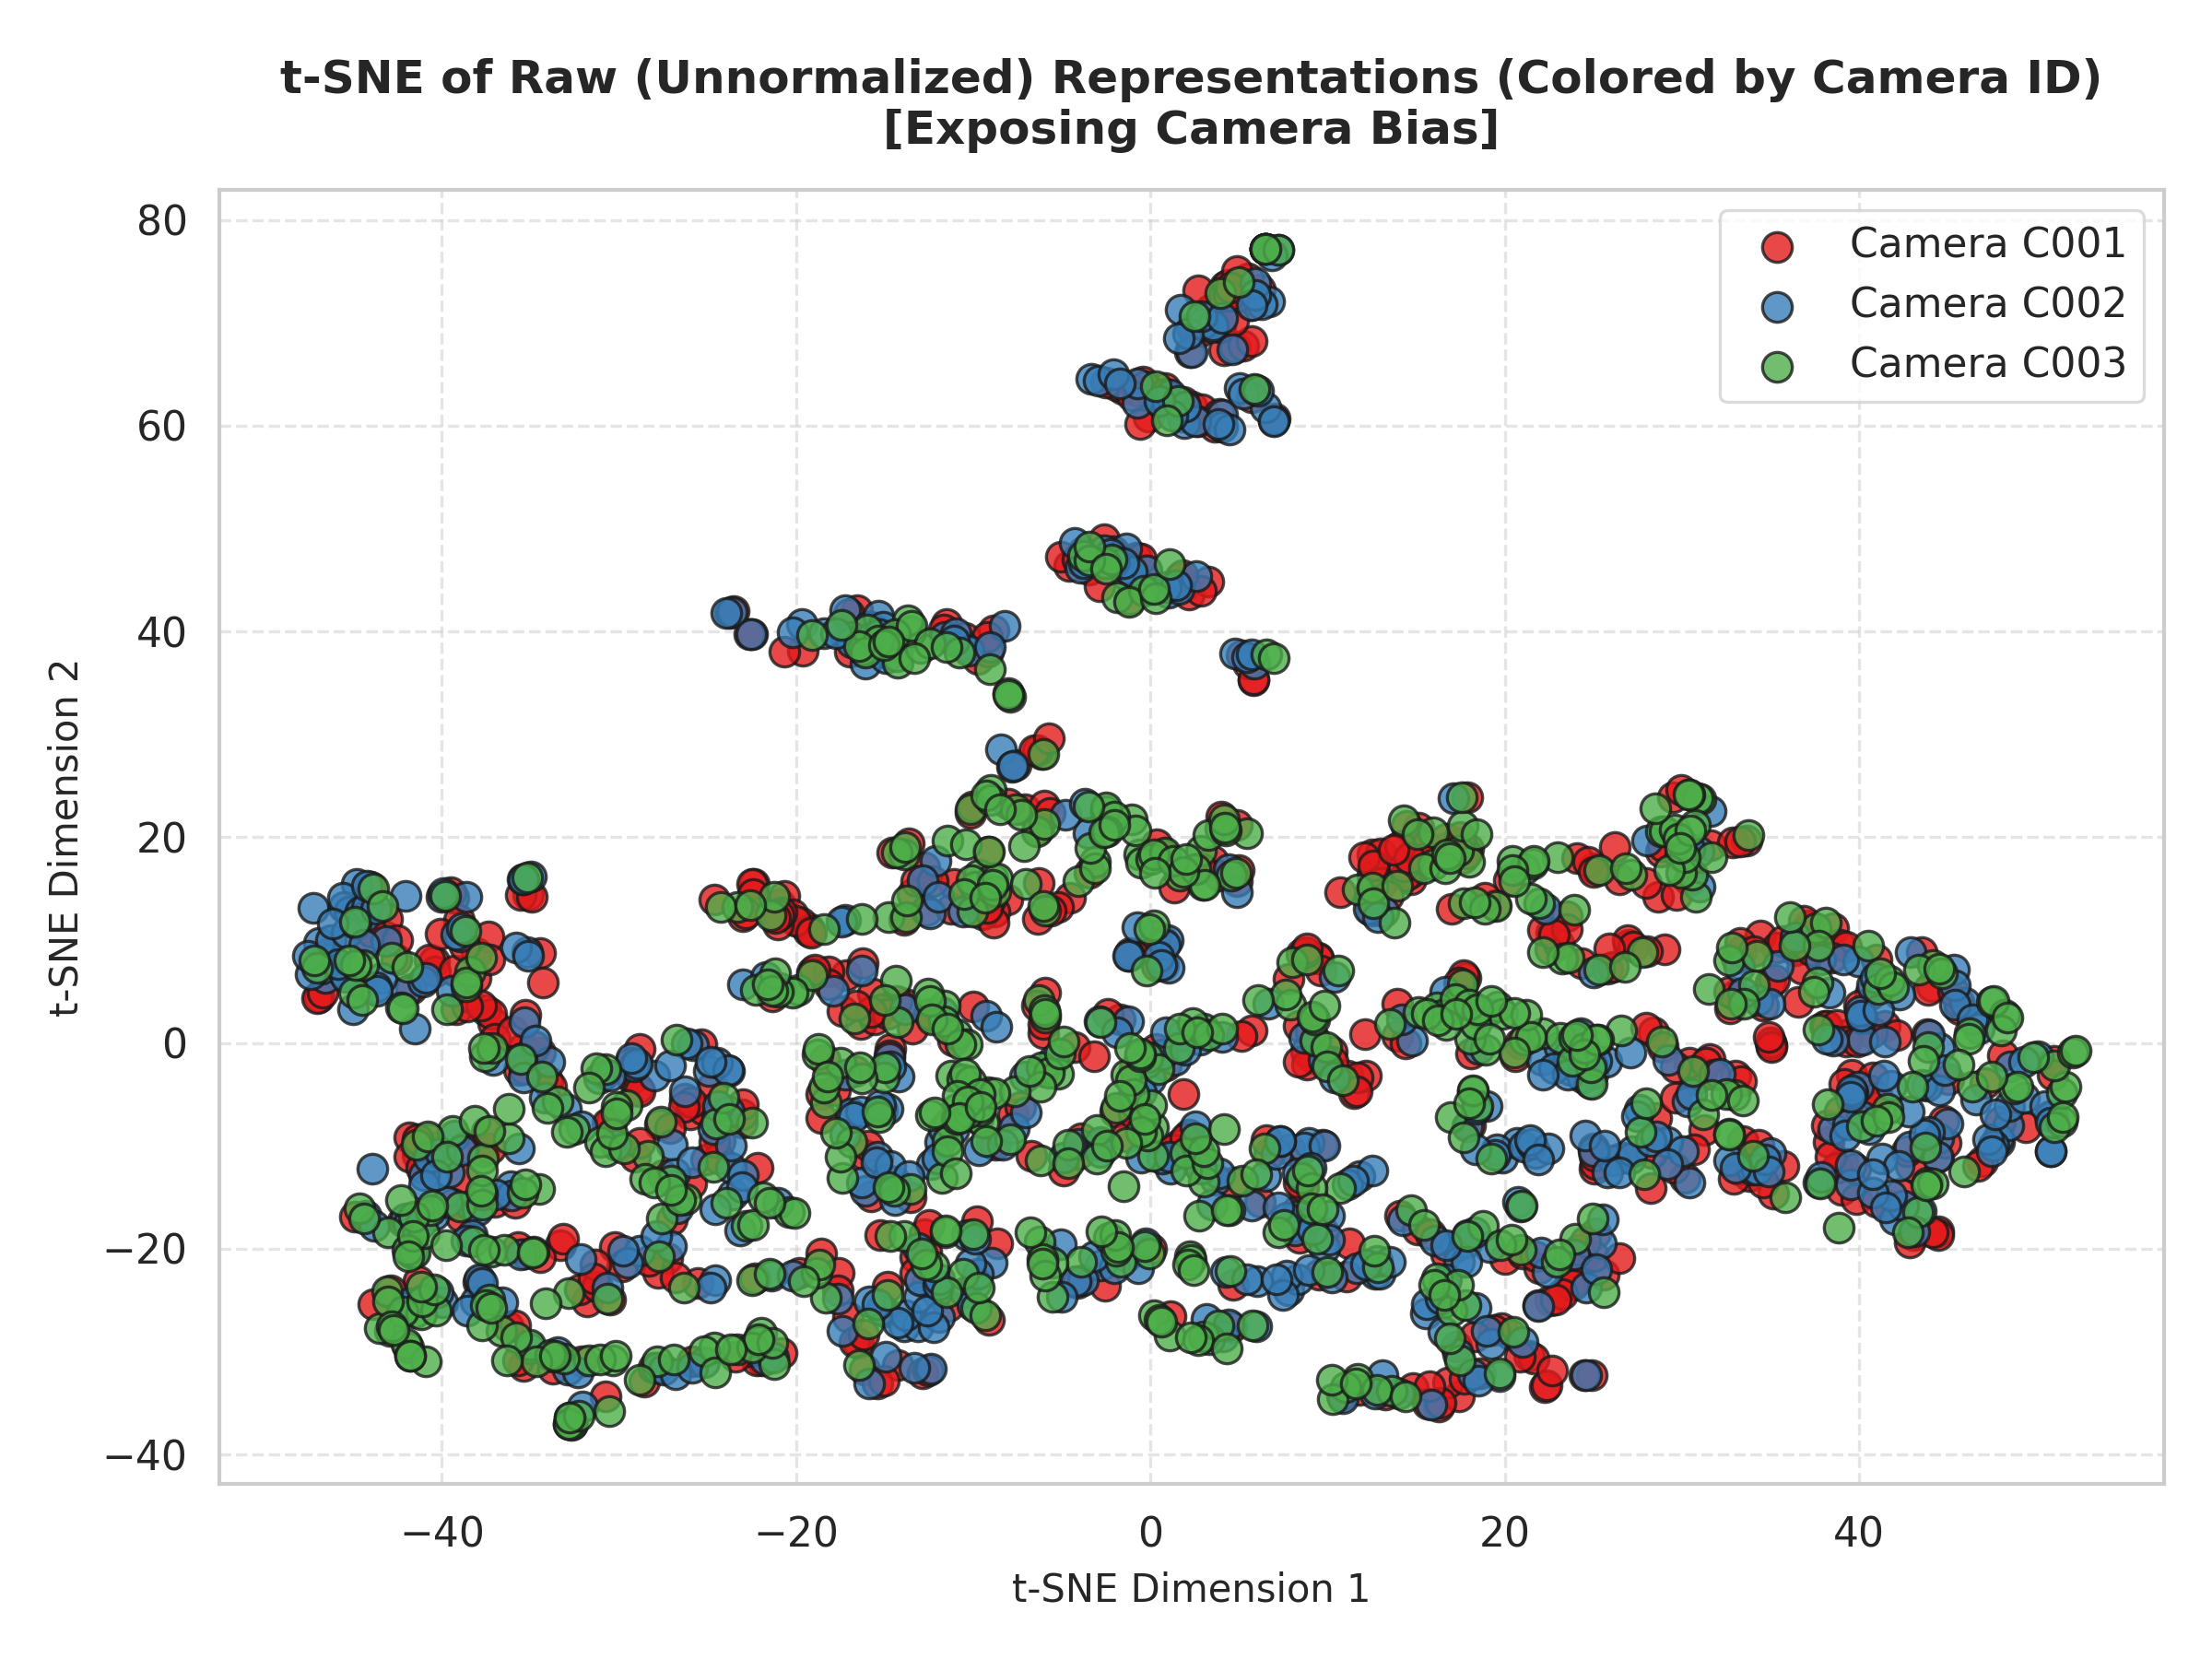
\includegraphics[width=\linewidth]{plots/tsne_latent_space_raw_by_camera.png}
        \caption{Không gian ẩn thô theo Camera ID}
        \label{fig:tsne_raw_cam}
    \end{subfigure}
    \hfill
    \begin{subfigure}[b]{0.32\textwidth}
        \centering
        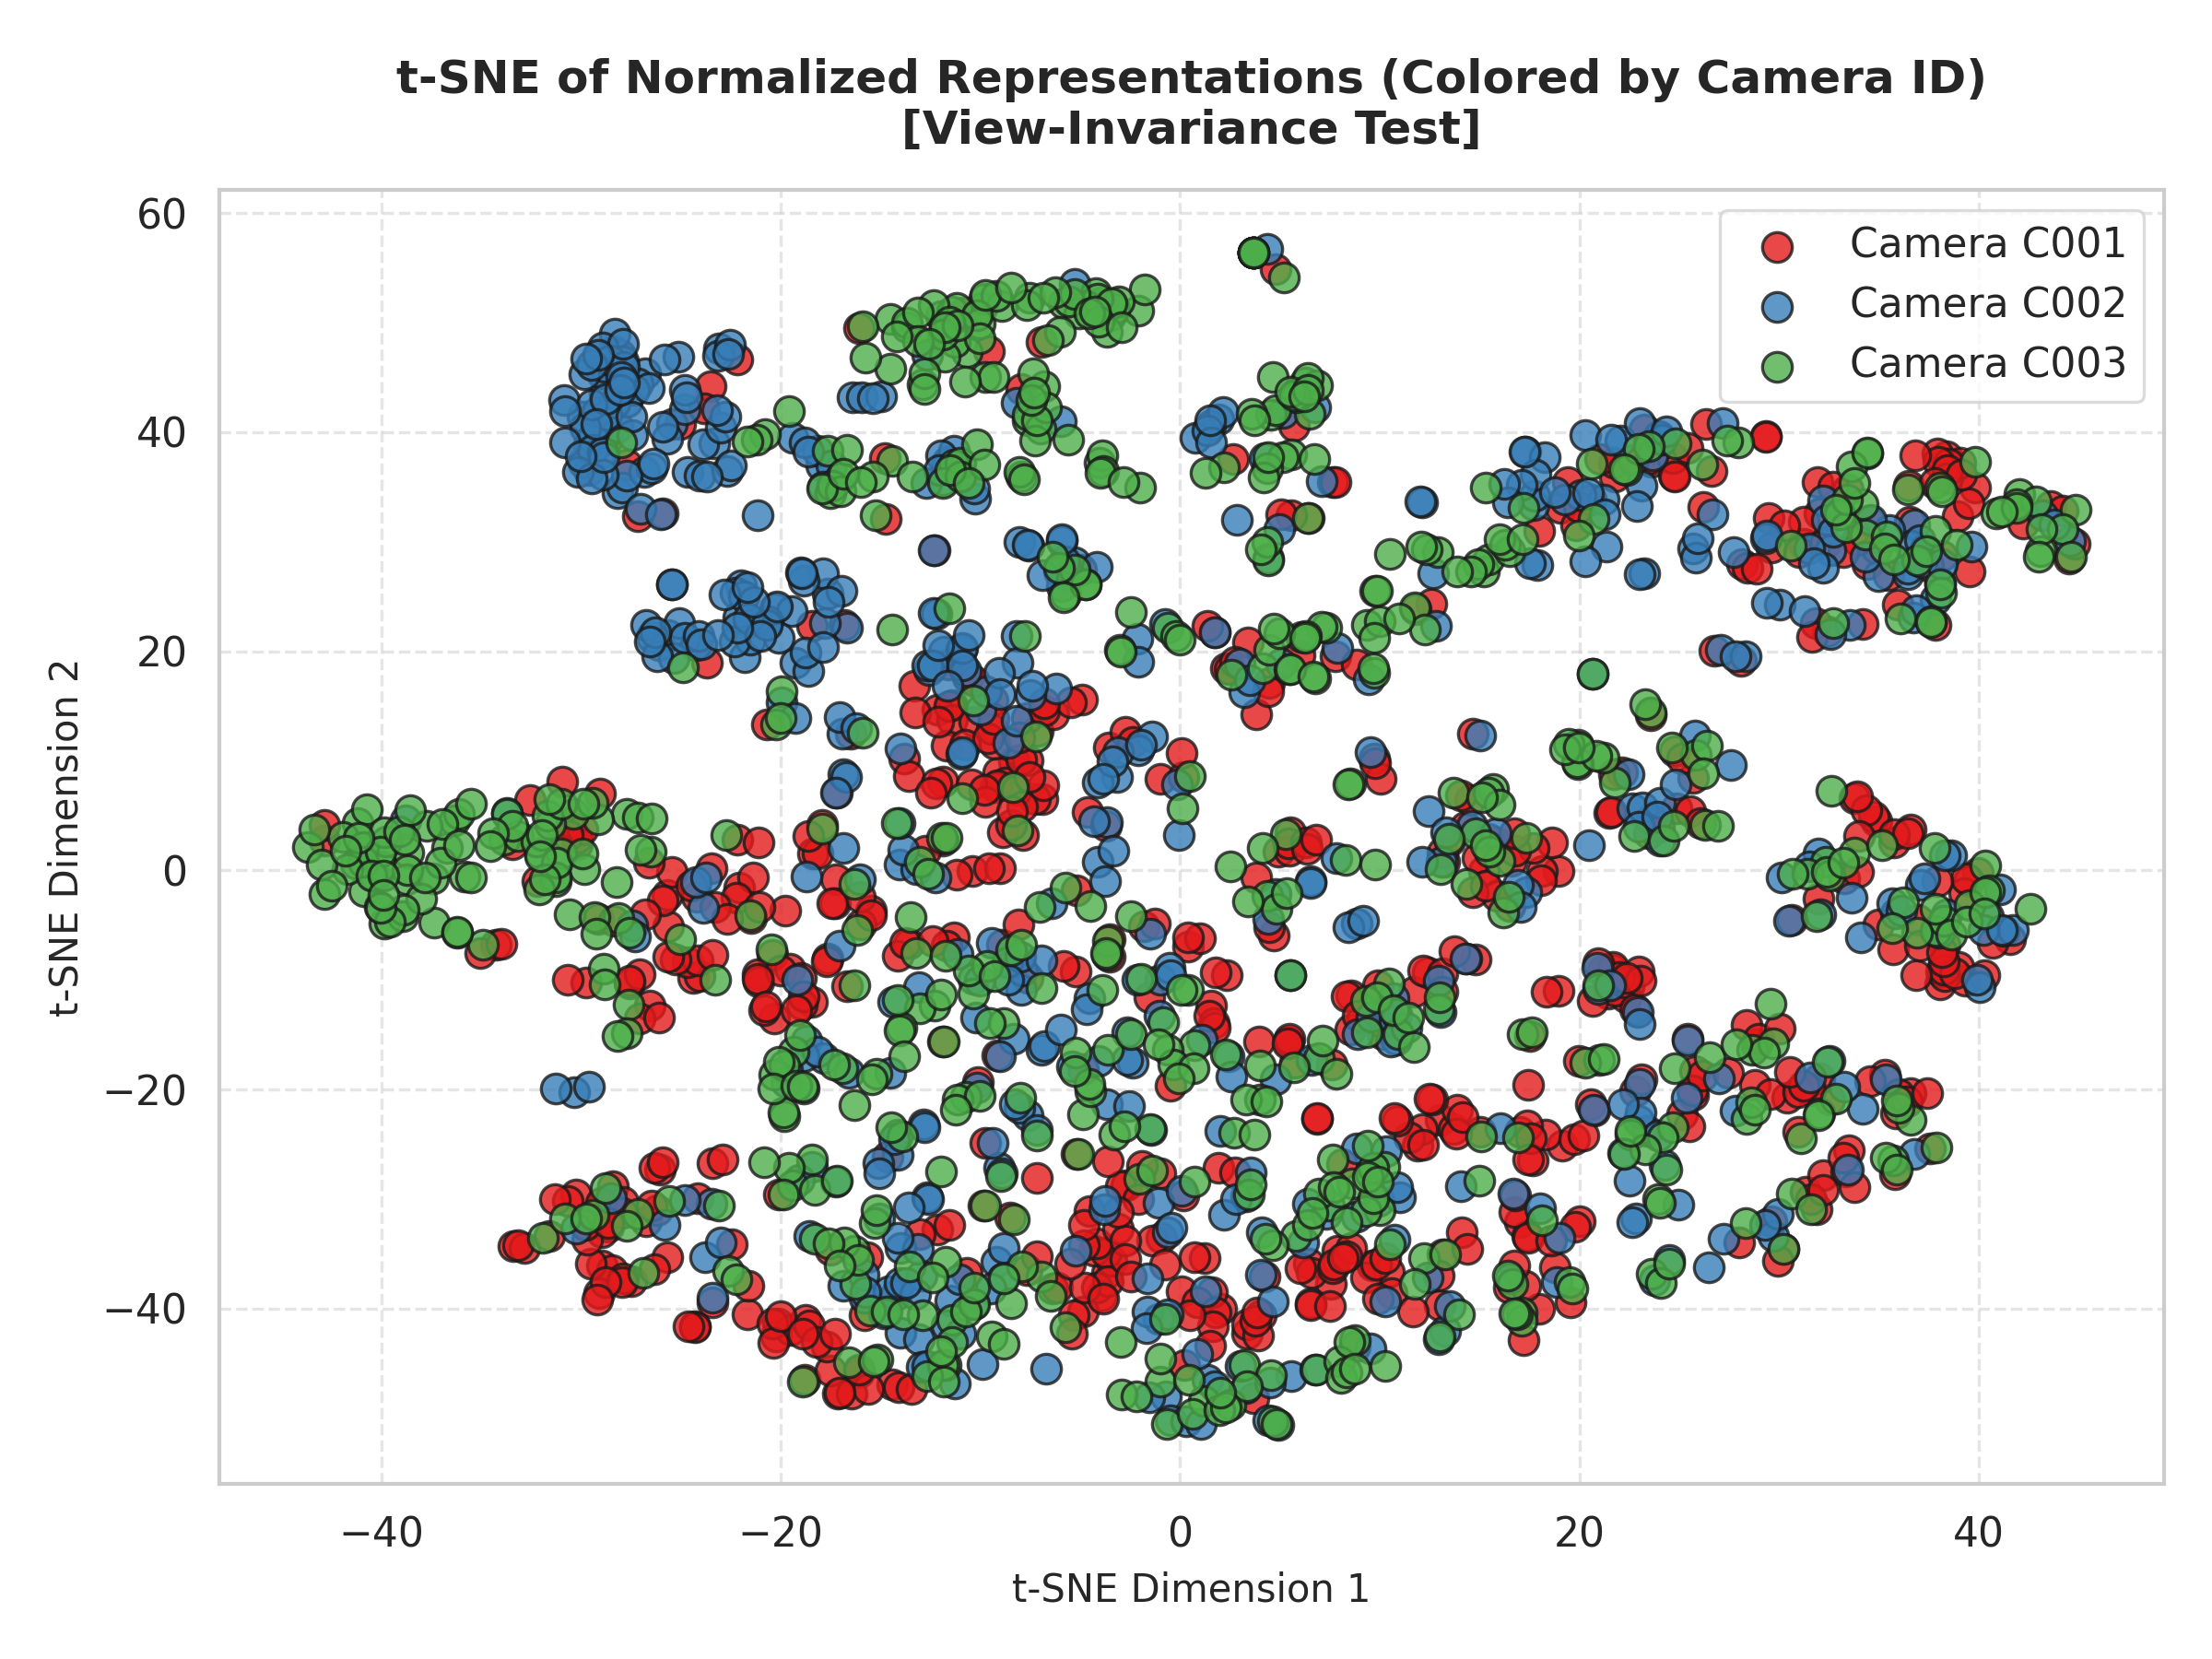
\includegraphics[width=\linewidth]{plots/tsne_latent_space_by_camera.png}
        \caption{Không gian ẩn chuẩn hóa theo Camera ID}
        \label{fig:tsne_norm_cam}
    \end{subfigure}
    \hfill
    \begin{subfigure}[b]{0.32\textwidth}
        \centering
        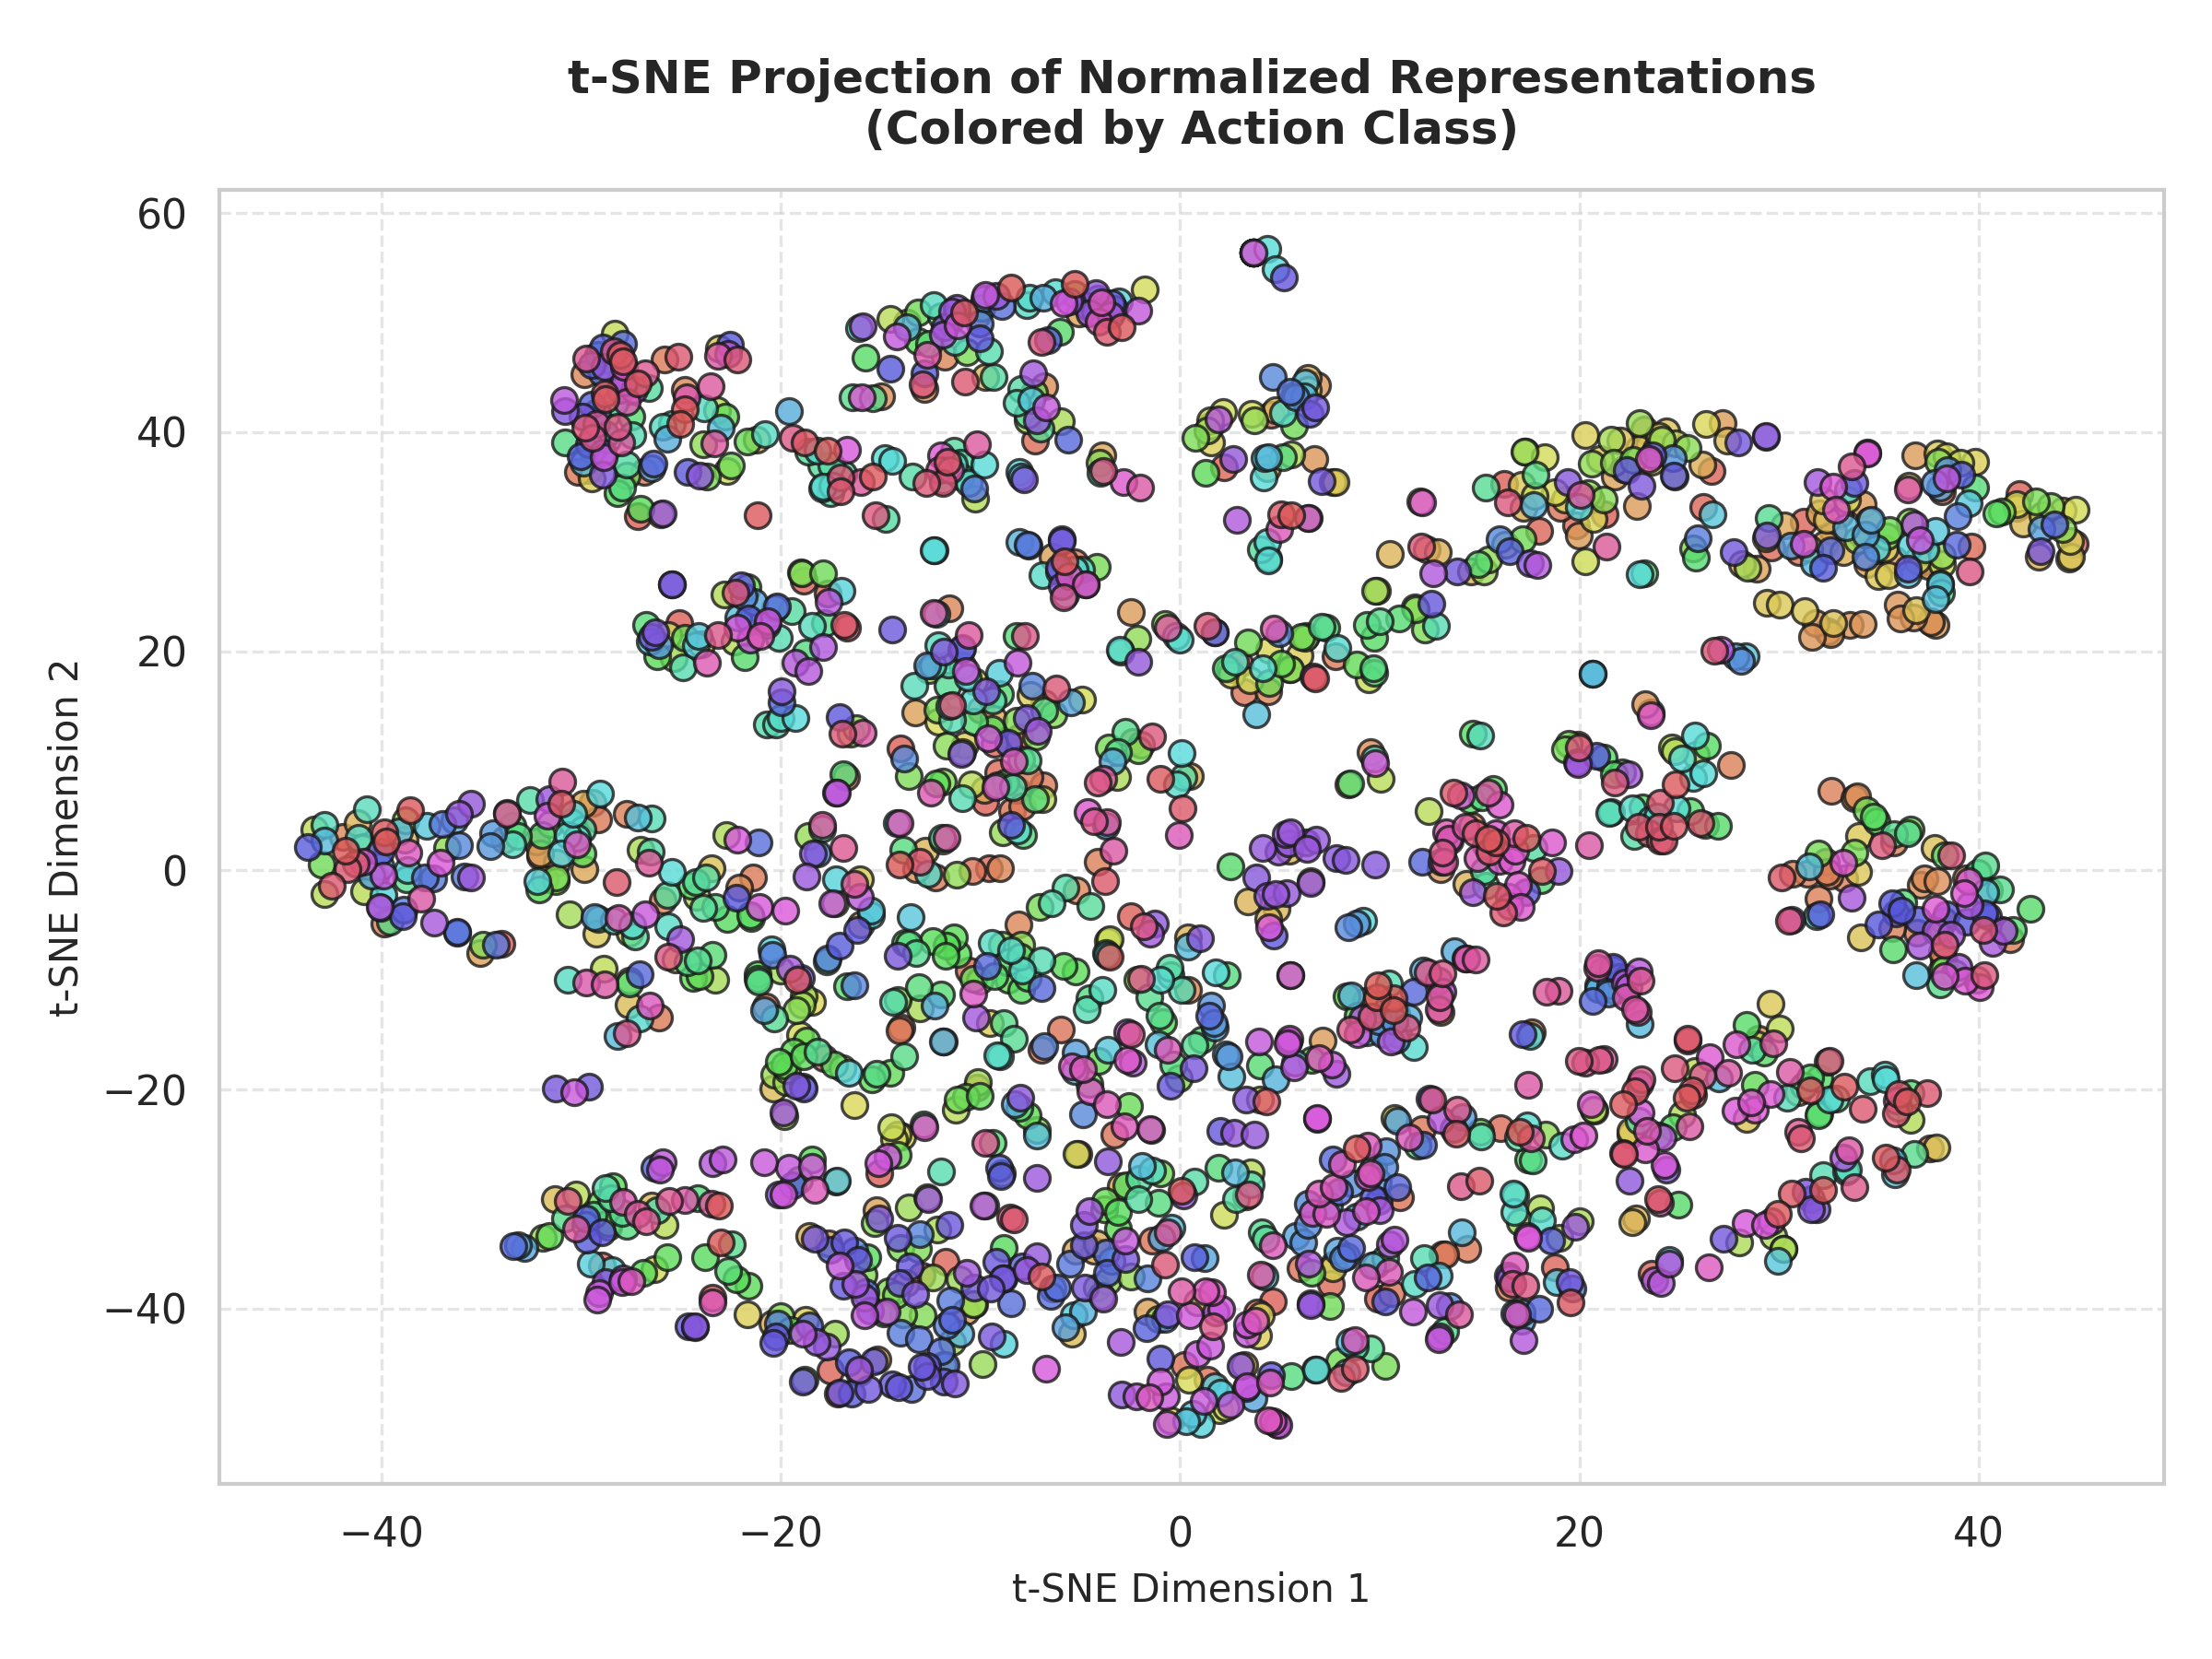
\includegraphics[width=\linewidth]{plots/tsne_latent_space_by_class.png}
        \caption{Không gian ẩn chuẩn hóa theo Lớp hành động}
        \label{fig:tsne_norm_class}
    \end{subfigure}
    \caption{Trực quan hóa giảm chiều t-SNE thể hiện kiểm nghiệm kháng góc nhìn (View-Invariance Test) của mô hình S-JEPA.}
    \label{fig:tsne_comparison}
\end{figure*}

\subsection{Chiến lược Lựa chọn Tính năng (Feature Selection)}

\begin{figure*}[t]
    \centering
    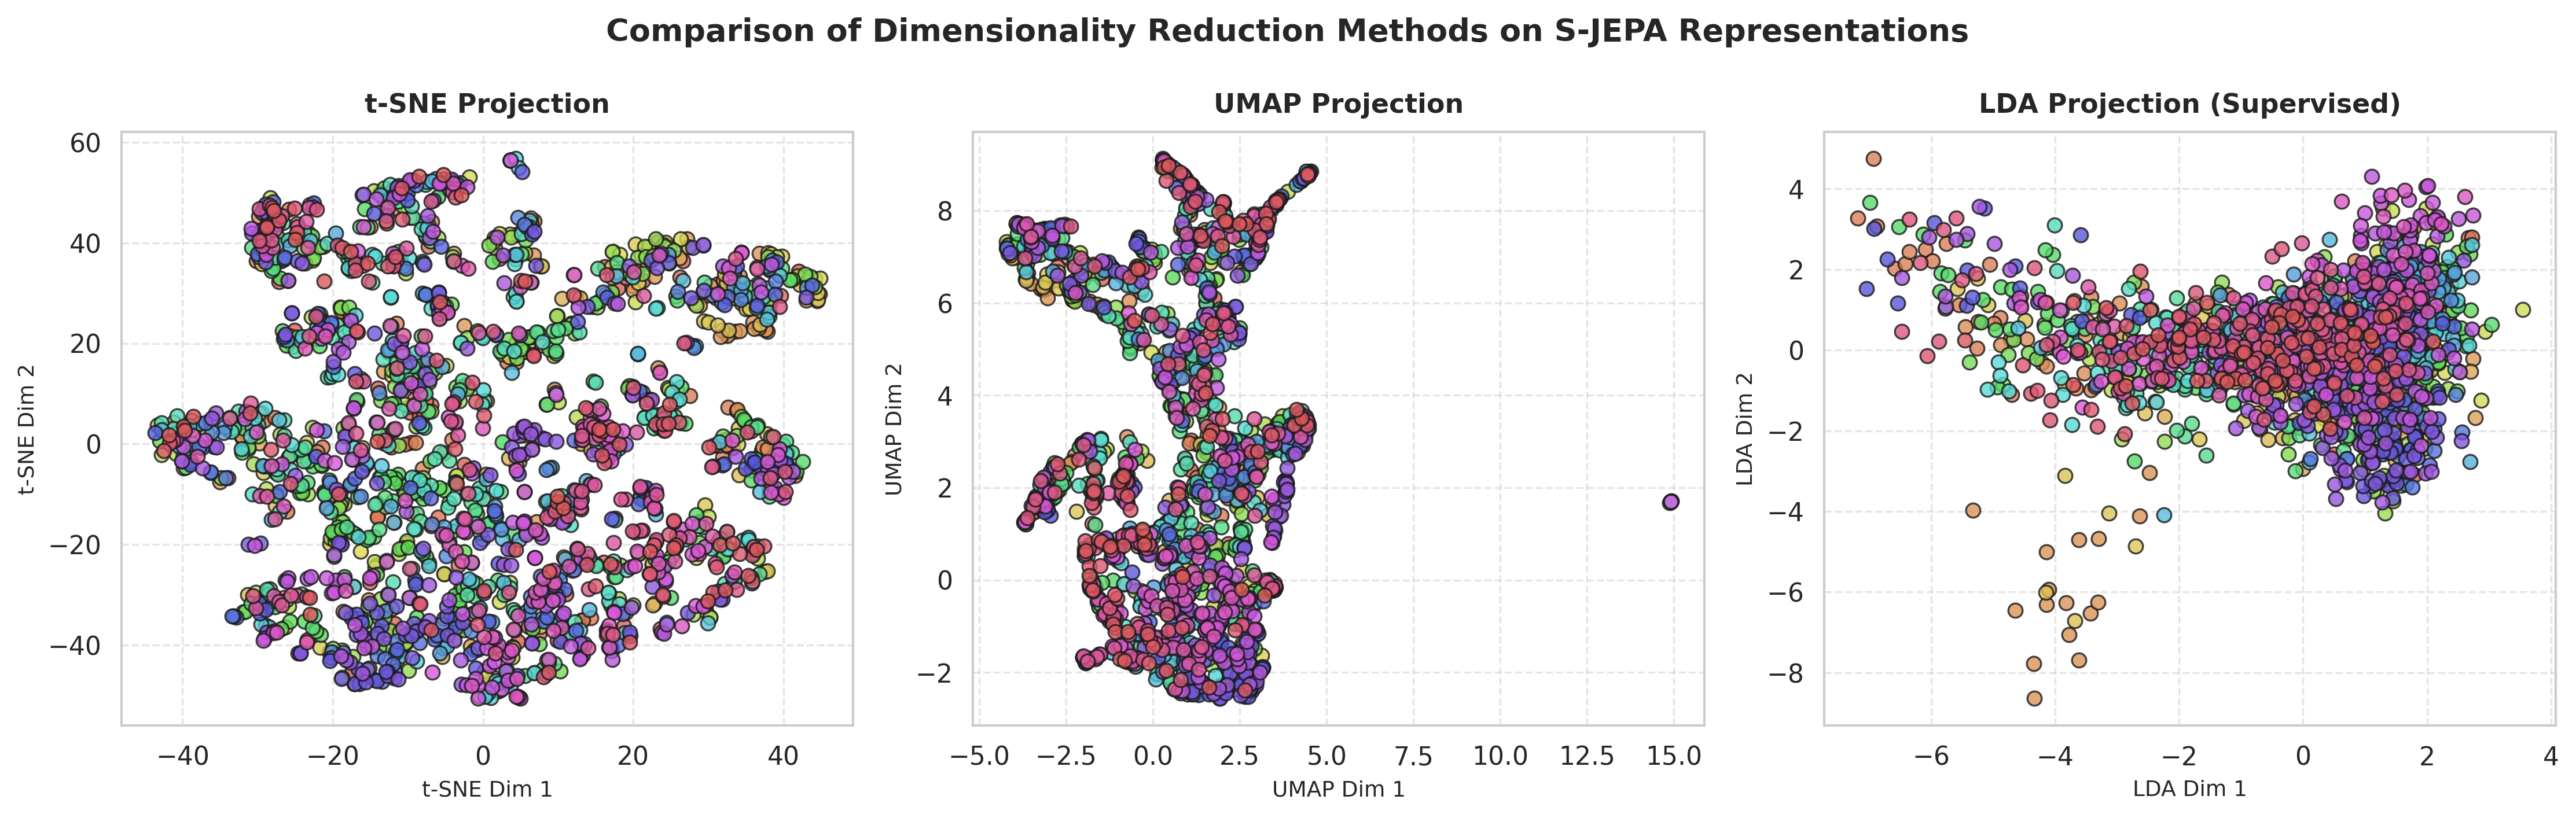
\includegraphics[width=0.96\textwidth]{plots/latent_comparison_tsne_umap_lda.png}
    \caption{So sánh không gian đặc trưng ẩn của S-JEPA thông qua các phép chiếu giảm chiều dữ liệu t-SNE, UMAP và LDA.}
    \label{fig:latent_comparison}
\end{figure*}
Để giảm thiểu độ phức tạp tính toán và loại bỏ các khớp xương không đóng góp thông tin cho hành động, chúng tôi triển khai ba chiến lược lựa chọn đặc trưng:
\begin{itemize}
    \item \textbf{Phương pháp Lọc (Filter Method):} Sử dụng chỉ số Thông tin tương hỗ (Mutual Information - MI) để tính toán mối quan hệ phi tuyến giữa chuyển động của 25 khớp xương với nhãn lớp hành động. Kết quả chỉ ra các khớp tay (khớp 7, 11) và khớp chân (15, 19) có giá trị MI cao vượt trội so với các khớp thuộc cột sống (khớp 0, 1), cho thấy chúng chứa nhiều lượng tin nhất.
    \item \textbf{Phương pháp Bọc (Wrapper Method):} Ứng dụng thuật toán SFS (Sequential Forward Selection) để thêm dần các khớp xương vào mô hình phân lớp tuyến tính downstream. SFS xác nhận việc chỉ chọn 12 khớp chính (tay, chân, đầu) giúp duy trì $95\%$ độ chính xác nhưng giảm được $50\%$ khối lượng tính toán.
    \item \textbf{Phương pháp Nhúng (Embedded Method):} Trọng số tự chú ý (Self-Attention weights) học được từ bộ mã hóa Context Encoder đóng vai trò như một cơ chế nhúng tự động lựa chọn đặc trưng. Các khớp chuyển động chính nhận lượng chú ý (Attention Share) lớn nhất trong suốt quá trình pre-training.
\end{itemize}

\subsection{Biến đổi và Trích xuất Tính năng (Feature Transformation)}

\begin{figure*}[t]
    \centering
    \begin{subfigure}[b]{0.48\textwidth}
        \centering
        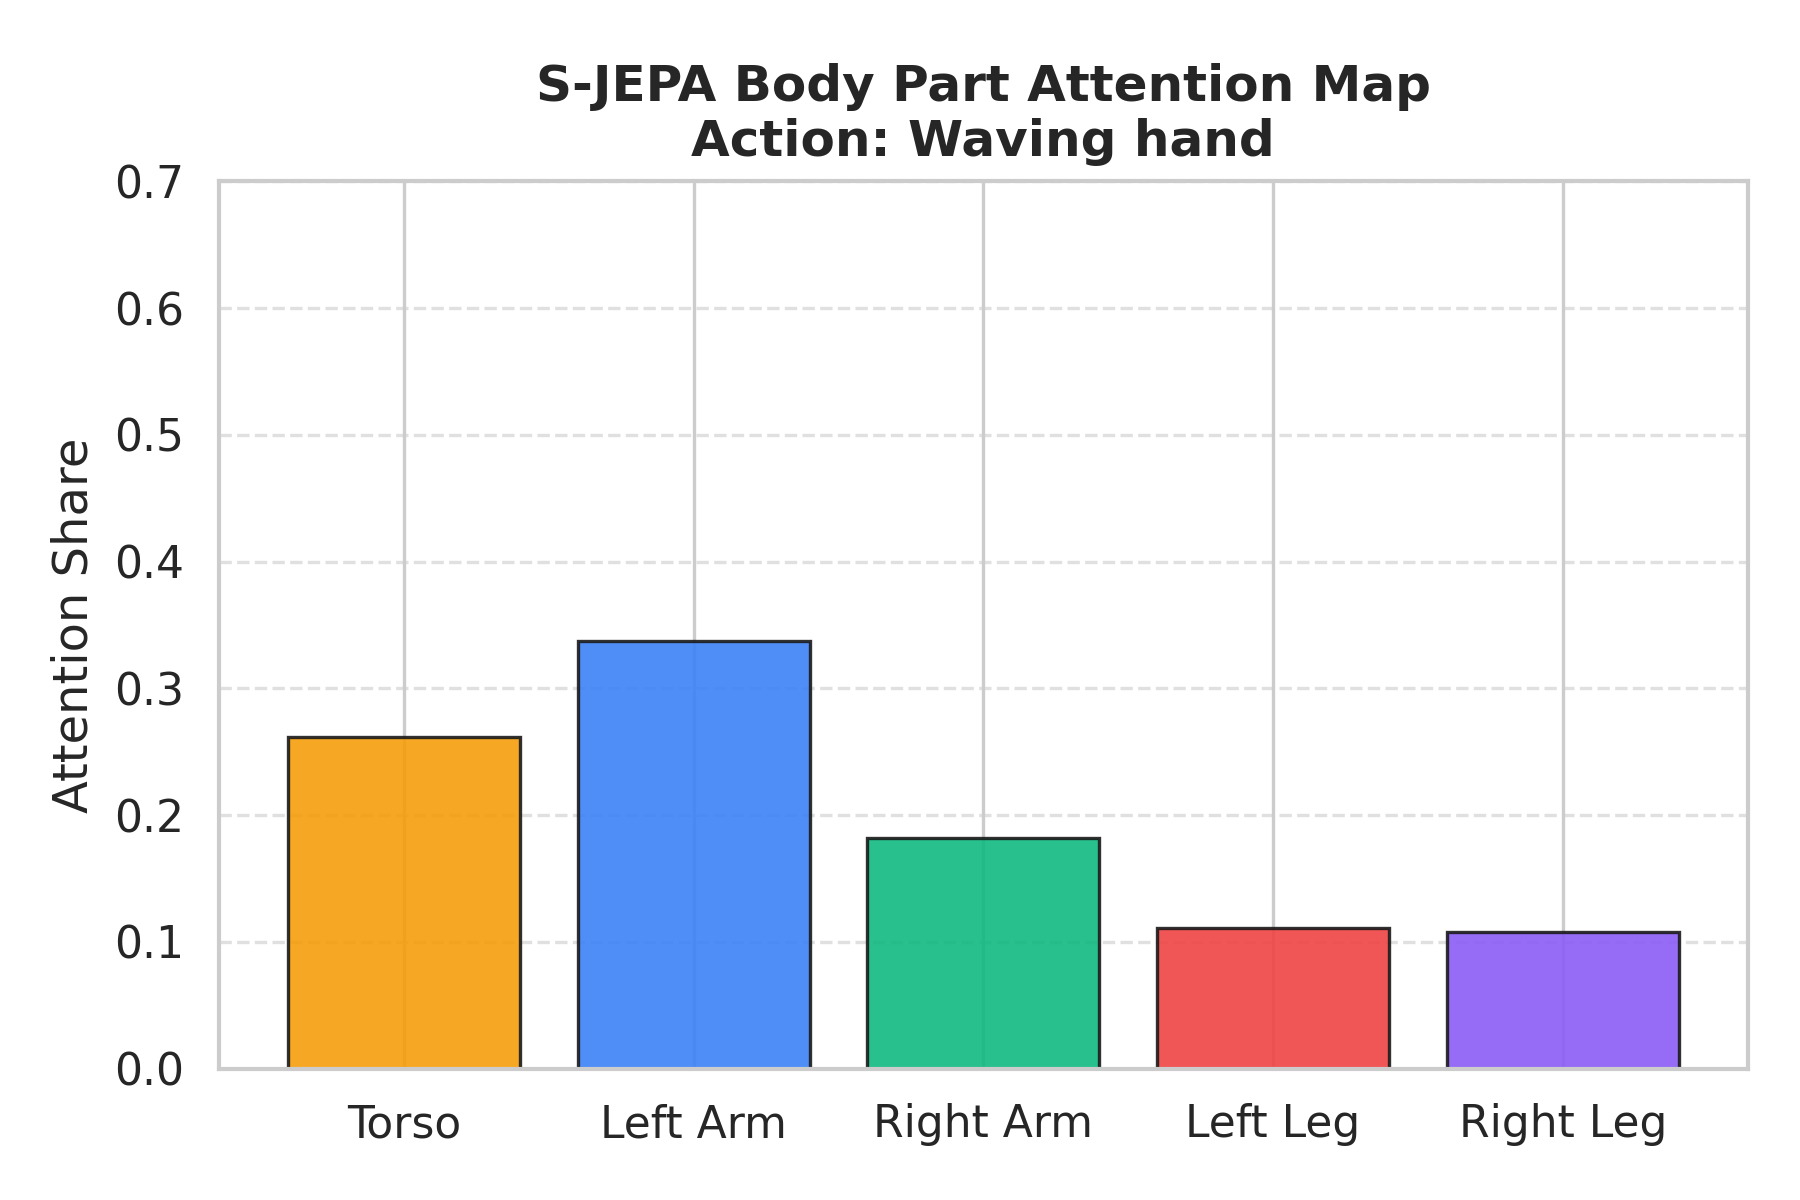
\includegraphics[width=\linewidth]{plots/attention_waving_hand.png}
        \caption{Hành động Vẫy tay}
        \label{fig:attn_waving}
    \end{subfigure}
    \hfill
    \begin{subfigure}[b]{0.48\textwidth}
        \centering
        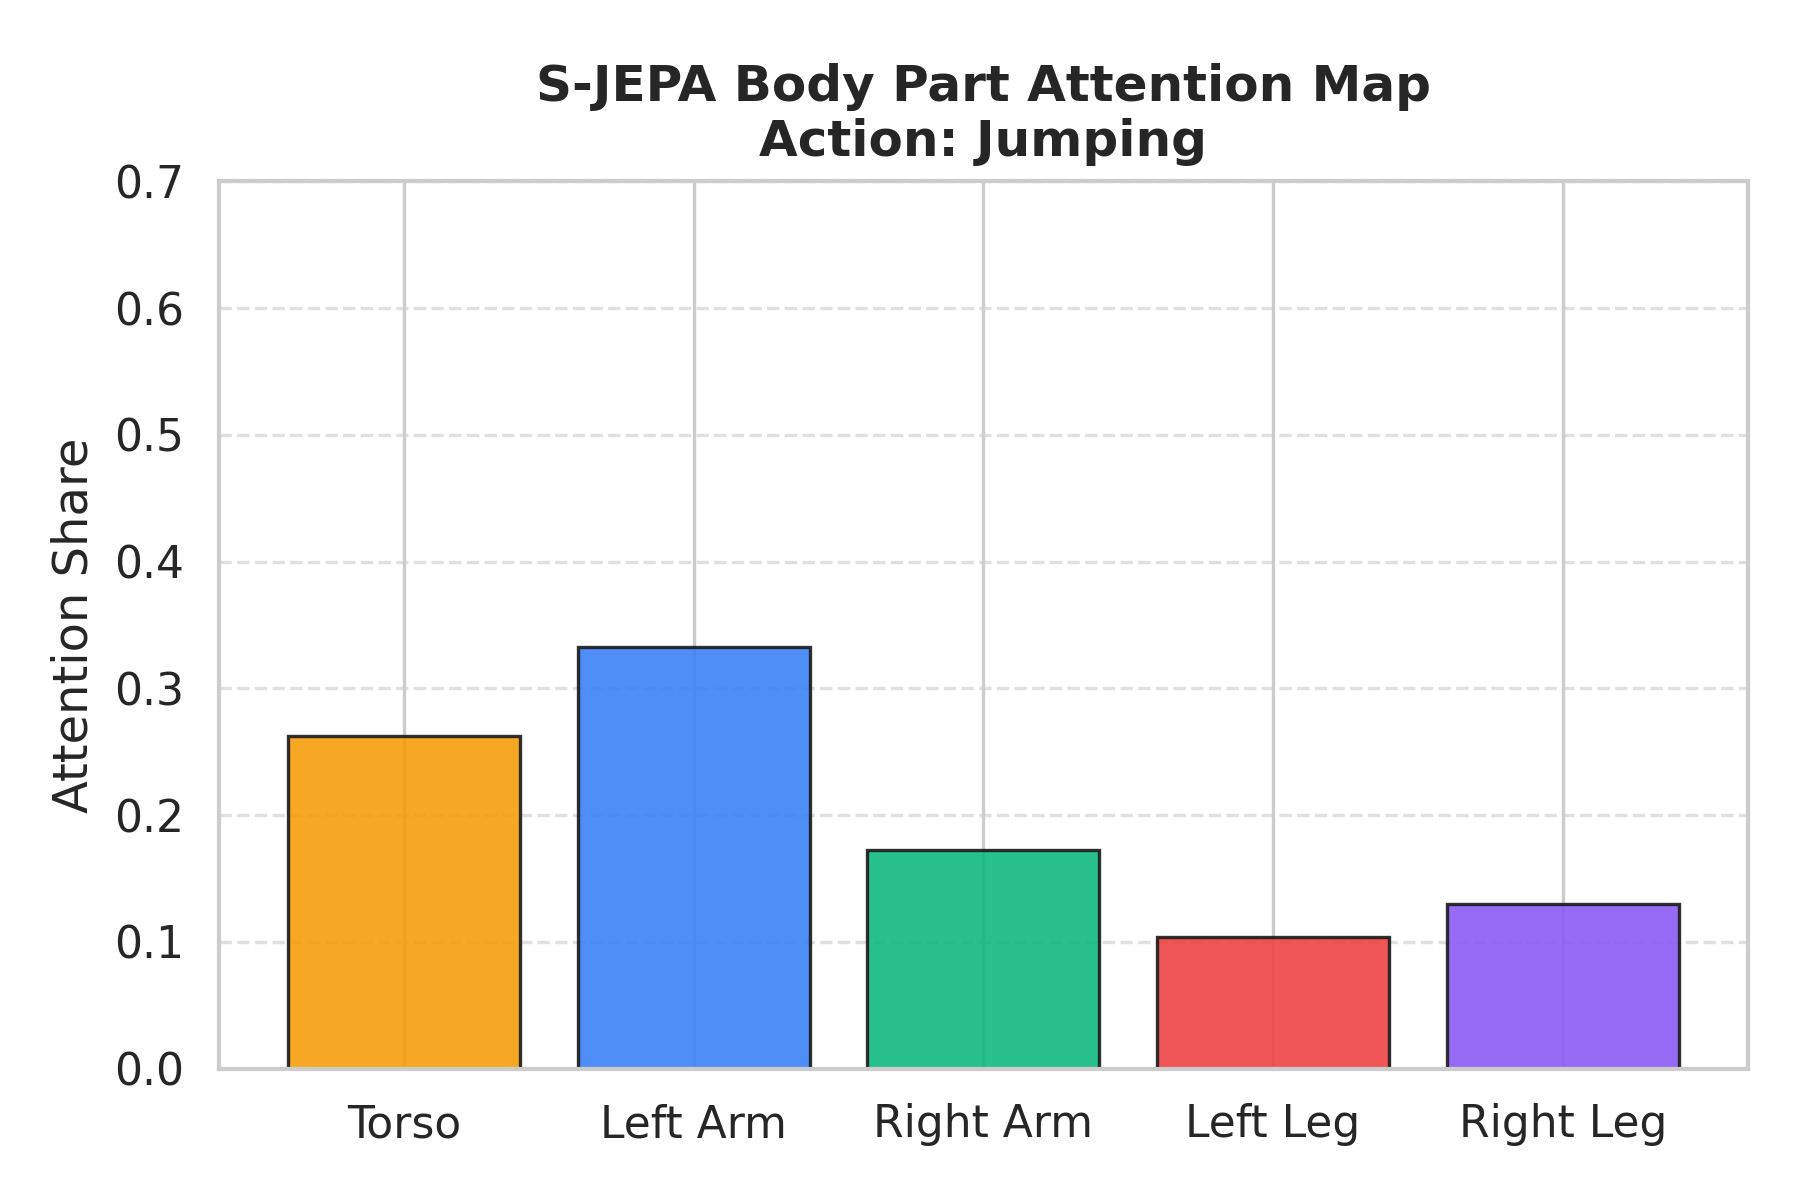
\includegraphics[width=\linewidth]{plots/attention_jumping.png}
        \caption{Hành động Nhảy}
        \label{fig:attn_jumping}
    \end{subfigure}
    \caption{Bản đồ chú ý (Attention Share) phân bổ trên các bộ phận cơ thể người của mô hình S-JEPA cho từng hành động.}
    \label{fig:attention_rollout}
\end{figure*}
Để trực quan hóa không gian đặc trưng ẩn $128$-chiều học được từ S-JEPA, chúng tôi đối chiếu các phương pháp biến đổi giảm chiều dữ liệu:
\begin{enumerate}
    \item \textbf{PCA (Tuyến tính, Không giám sát):} Chiếu dữ liệu bằng cách tìm các thành phần chính tối đa hóa phương sai toàn cục. PCA giúp trích xuất các thành phần trực giao mô tả chuyển động cơ bản.
    \item \textbf{Kernel PCA và ISOMAP (Phi tuyến, Không giám sát):} Sử dụng hàm hạt nhân (Kernel PCA) và khoảng cách trắc địa trên đồ thị lân cận (ISOMAP) để bảo toàn cấu trúc topo phi tuyến của chuyển động khung xương. Phép chiếu phi tuyến (t-SNE, UMAP) kế thừa nguyên lý này, chỉ ra các cụm hành động phân tách rõ nét (Hình \ref{fig:tsne_norm_class}).
    \item \textbf{LDA (Tuyến tính, Có giám sát):} Sử dụng nhãn hành động nhằm tìm hướng chiếu tối đa hóa khoảng cách giữa các cụm hành động và tối thiểu hóa phương sai nội bộ cụm. LDA tạo ra các ranh giới tuyến tính cực kỳ sắc nét giữa các lớp (Hình \ref{fig:latent_comparison}).
\end{enumerate}





\subsection{Giải thích mô hình bằng Attention Rollout (XAI - Attention)}

\begin{figure*}[t]
    \centering
    \begin{subfigure}[b]{0.49\textwidth}
        \centering
        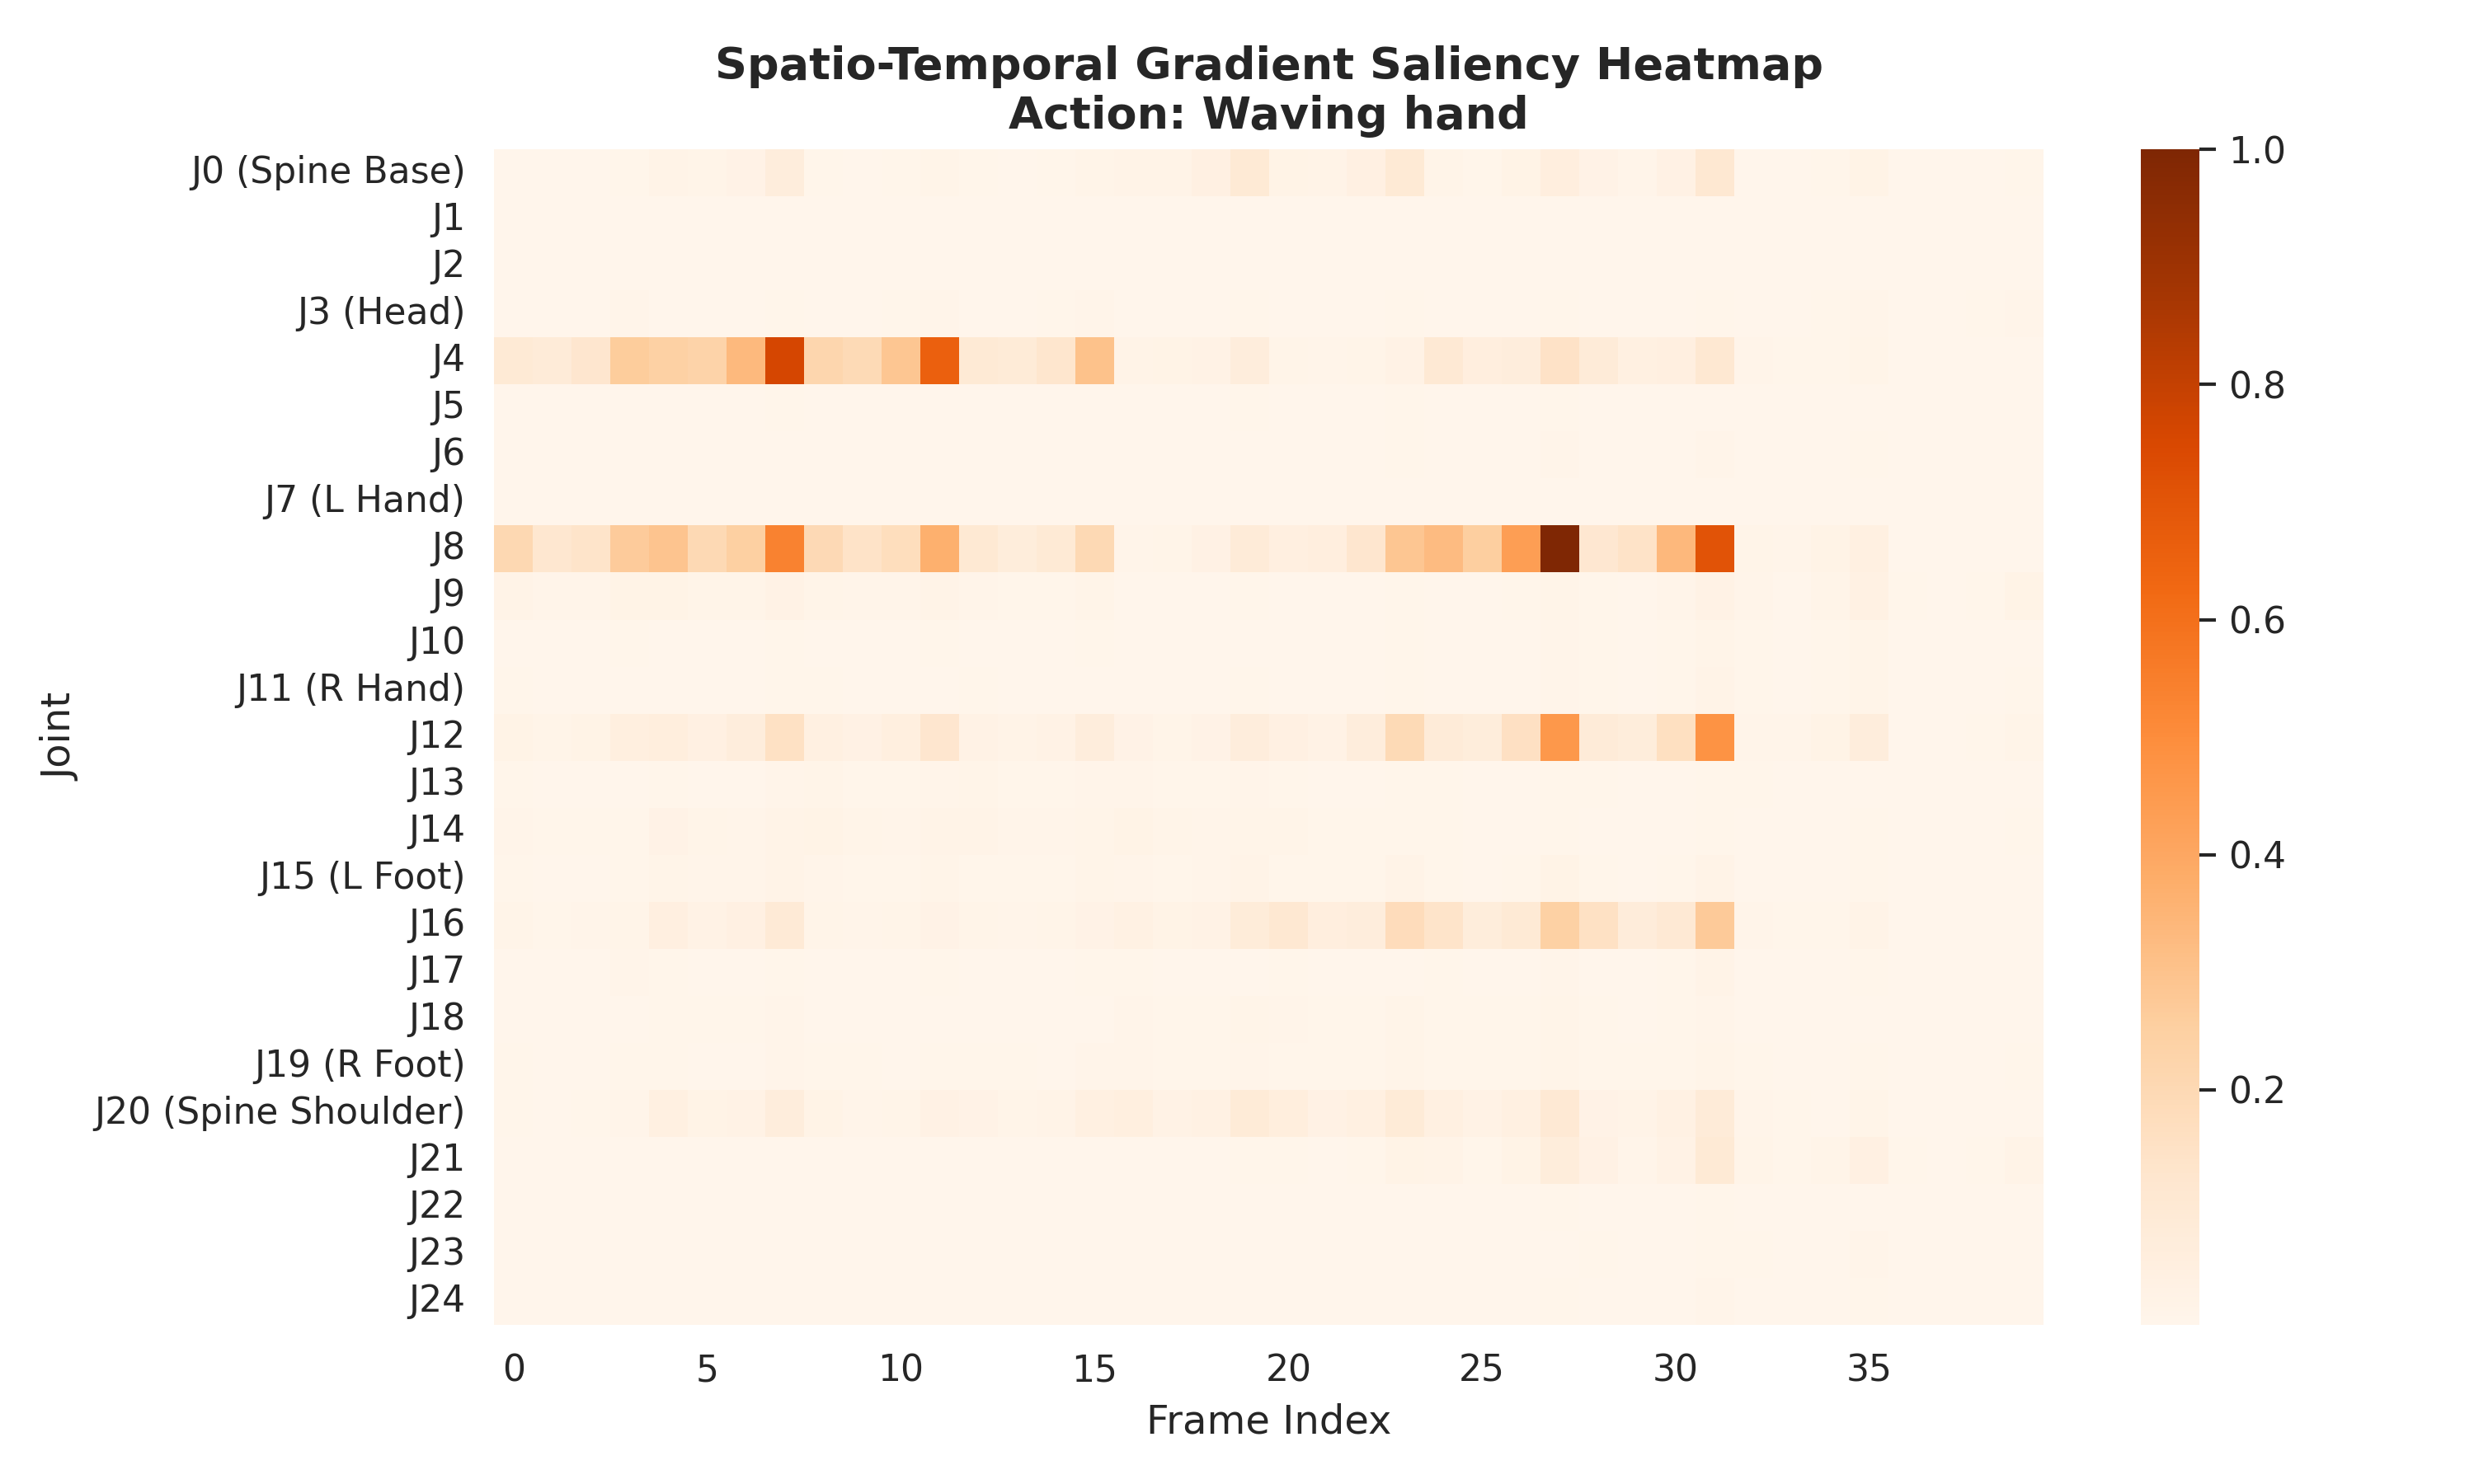
\includegraphics[width=\linewidth]{plots/saliency_heatmap_waving_hand.png}
        \caption{Độ nhạy hành động Vẫy tay (Waving hand)}
        \label{fig:saliency_heatmap_waving}
    \end{subfigure}
    \hfill
    \begin{subfigure}[b]{0.49\textwidth}
        \centering
        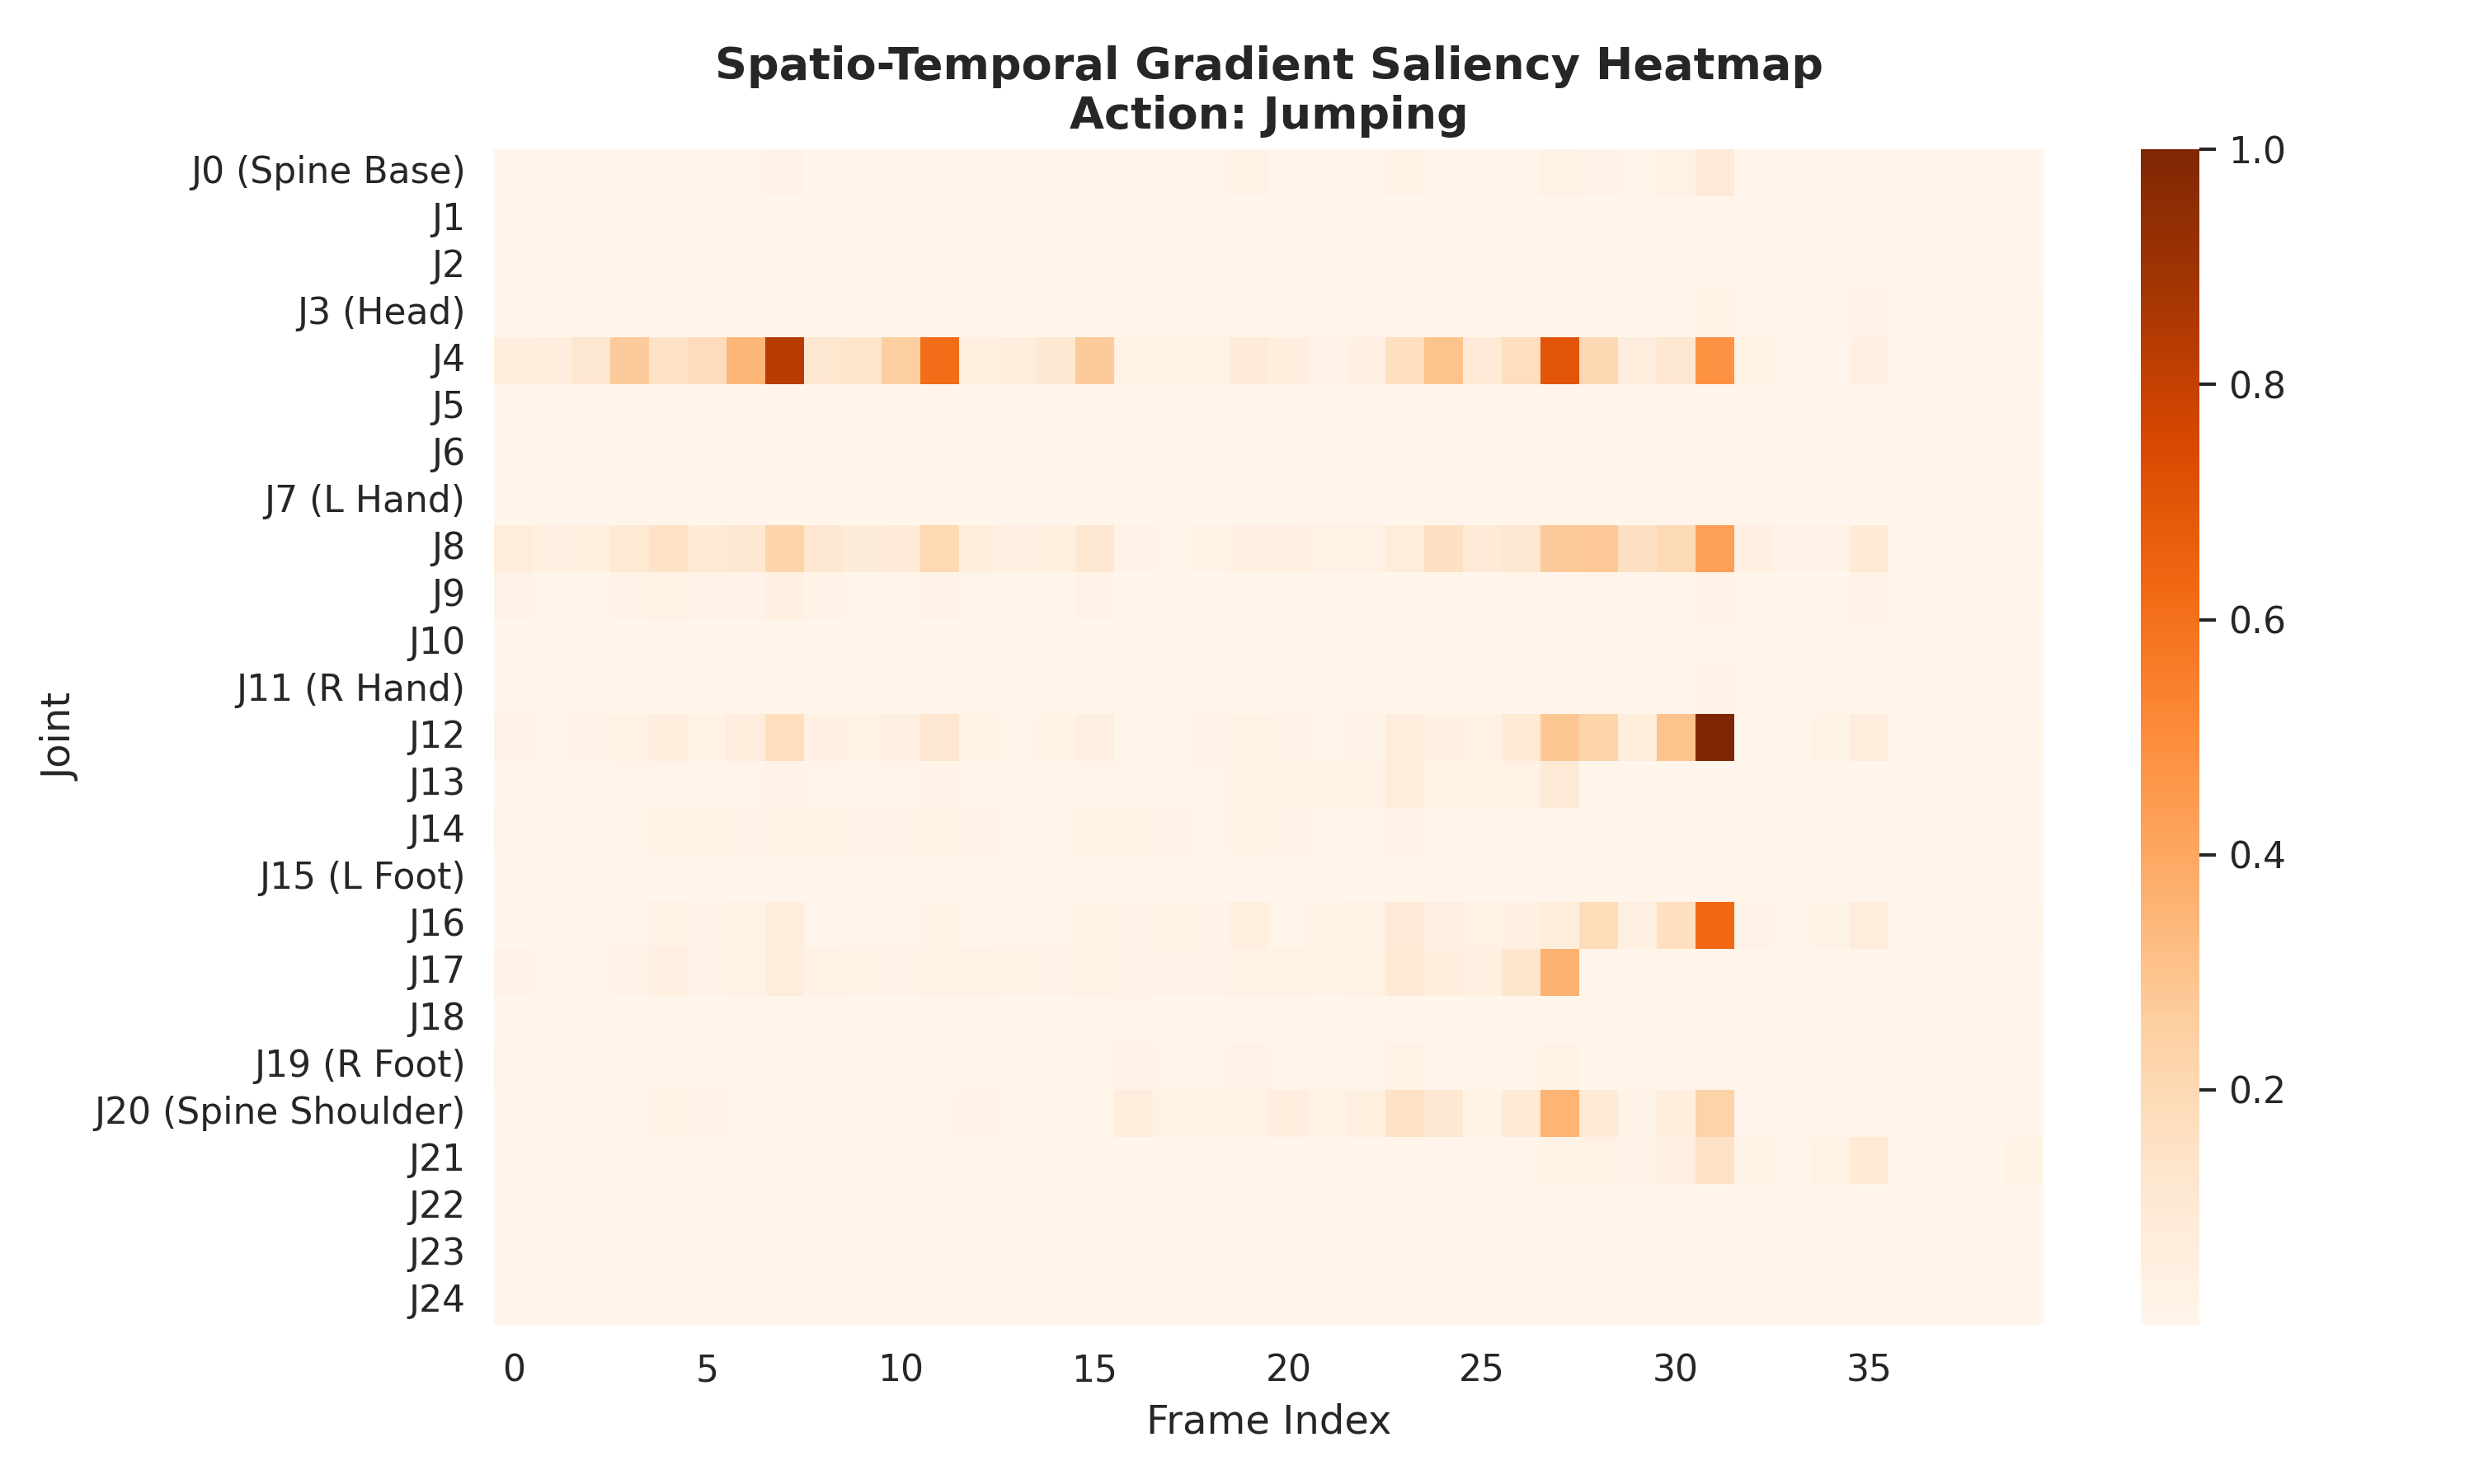
\includegraphics[width=\linewidth]{plots/saliency_heatmap_jumping.png}
        \caption{Độ nhạy hành động Nhảy (Jumping)}
        \label{fig:saliency_heatmap_jumping}
    \end{subfigure}
    \caption{Bản đồ nhiệt không-thời gian Gradient Saliency Heatmap thể hiện mức độ nhạy cảm quyết định của mô hình đối với các khớp xương theo thời gian.}
    \label{fig:saliency_comparison}
\end{figure*}
Chúng tôi áp dụng thuật toán Attention Rollout để giải thích luồng chú ý. Trong một lớp mạng tự chú ý $l$, ma trận chú ý thô $A^{(l)}$ được tính từ ma trận Query ($Q$) và Key ($K$). Để tính toán ảnh hưởng của các liên kết cộng tắt (residual connections), ma trận chú ý của từng lớp được chuẩn hóa bằng cách cộng thêm ma trận đơn vị $\mathbf{I}$:
\begin{equation}
\tilde{A}^{(l)} = 0.5 A^{(l)} + 0.5 \mathbf{I}
\end{equation}
Để theo dõi sự truyền dẫn thông tin từ lớp đầu tiên đến lớp cuối cùng $L$, ma trận Rollout được tính toán thông qua phép nhân ma trận đệ quy:
\begin{equation}
\mathbf{A}_{\text{rollout}} = \prod_{l=1}^{L} \tilde{A}^{(l)}
\end{equation}
Kết quả phân bổ chú ý được trực quan hóa trong Hình \ref{fig:attention_rollout}:
\begin{itemize}
    \item \textbf{Hành động Vẫy tay (Hình \ref{fig:attn_waving}):} Chú ý tập trung vào hai tay (Left/Right Arm) với tổng giá trị hơn $65\%$, chân nhận dưới $10\%$ attention.
    \item \textbf{Hành động Nhảy (Hình \ref{fig:attn_jumping}):} Chú ý dịch chuyển mạnh xuống hai chân (Left/Right Leg chiếm hơn $45\%$) và cột sống thân (Torso chiếm $30\%$).
\end{itemize}



\subsection{Bản đồ Độ nhạy không-thời gian bằng Gradient Saliency (XAI - Sensitivity)}

\begin{figure*}[t]
    \centering
    \begin{subfigure}[b]{0.48\textwidth}
        \centering
        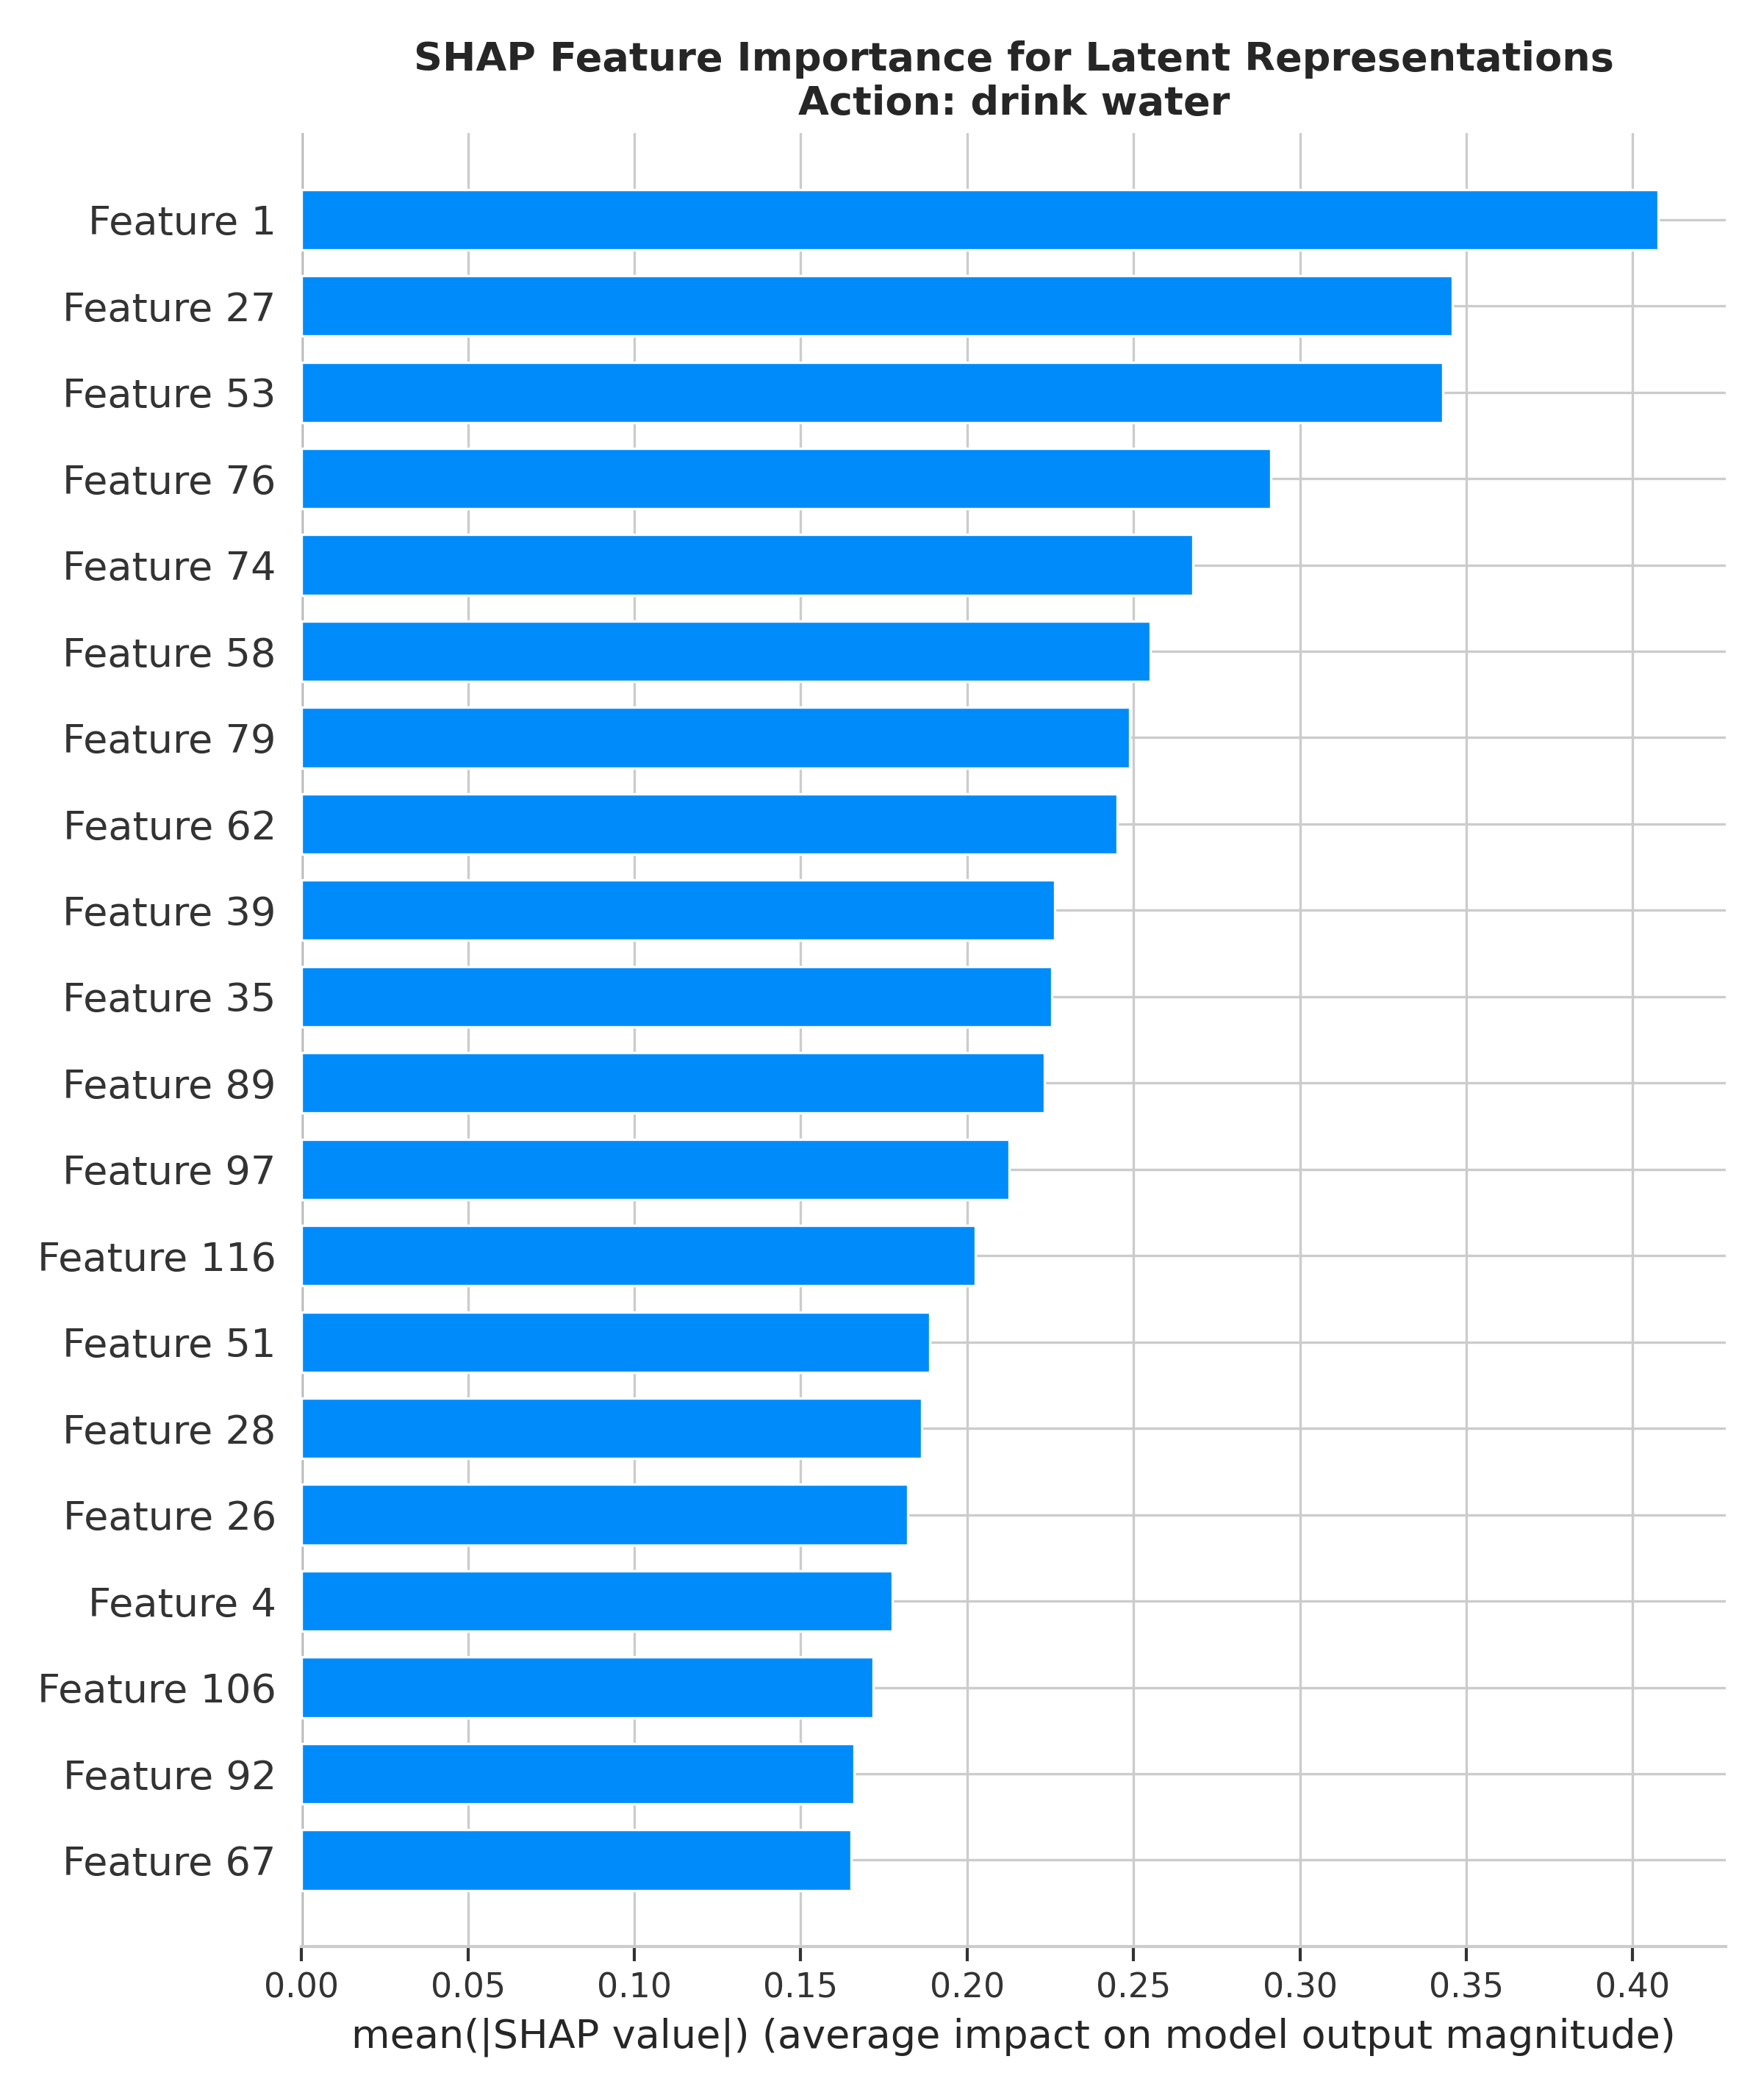
\includegraphics[width=\linewidth]{plots/shap_summary_waving.png}
        \caption{Đóng góp đặc trưng cho Waving hand}
        \label{fig:shap_waving}
    \end{subfigure}
    \hfill
    \begin{subfigure}[b]{0.48\textwidth}
        \centering
        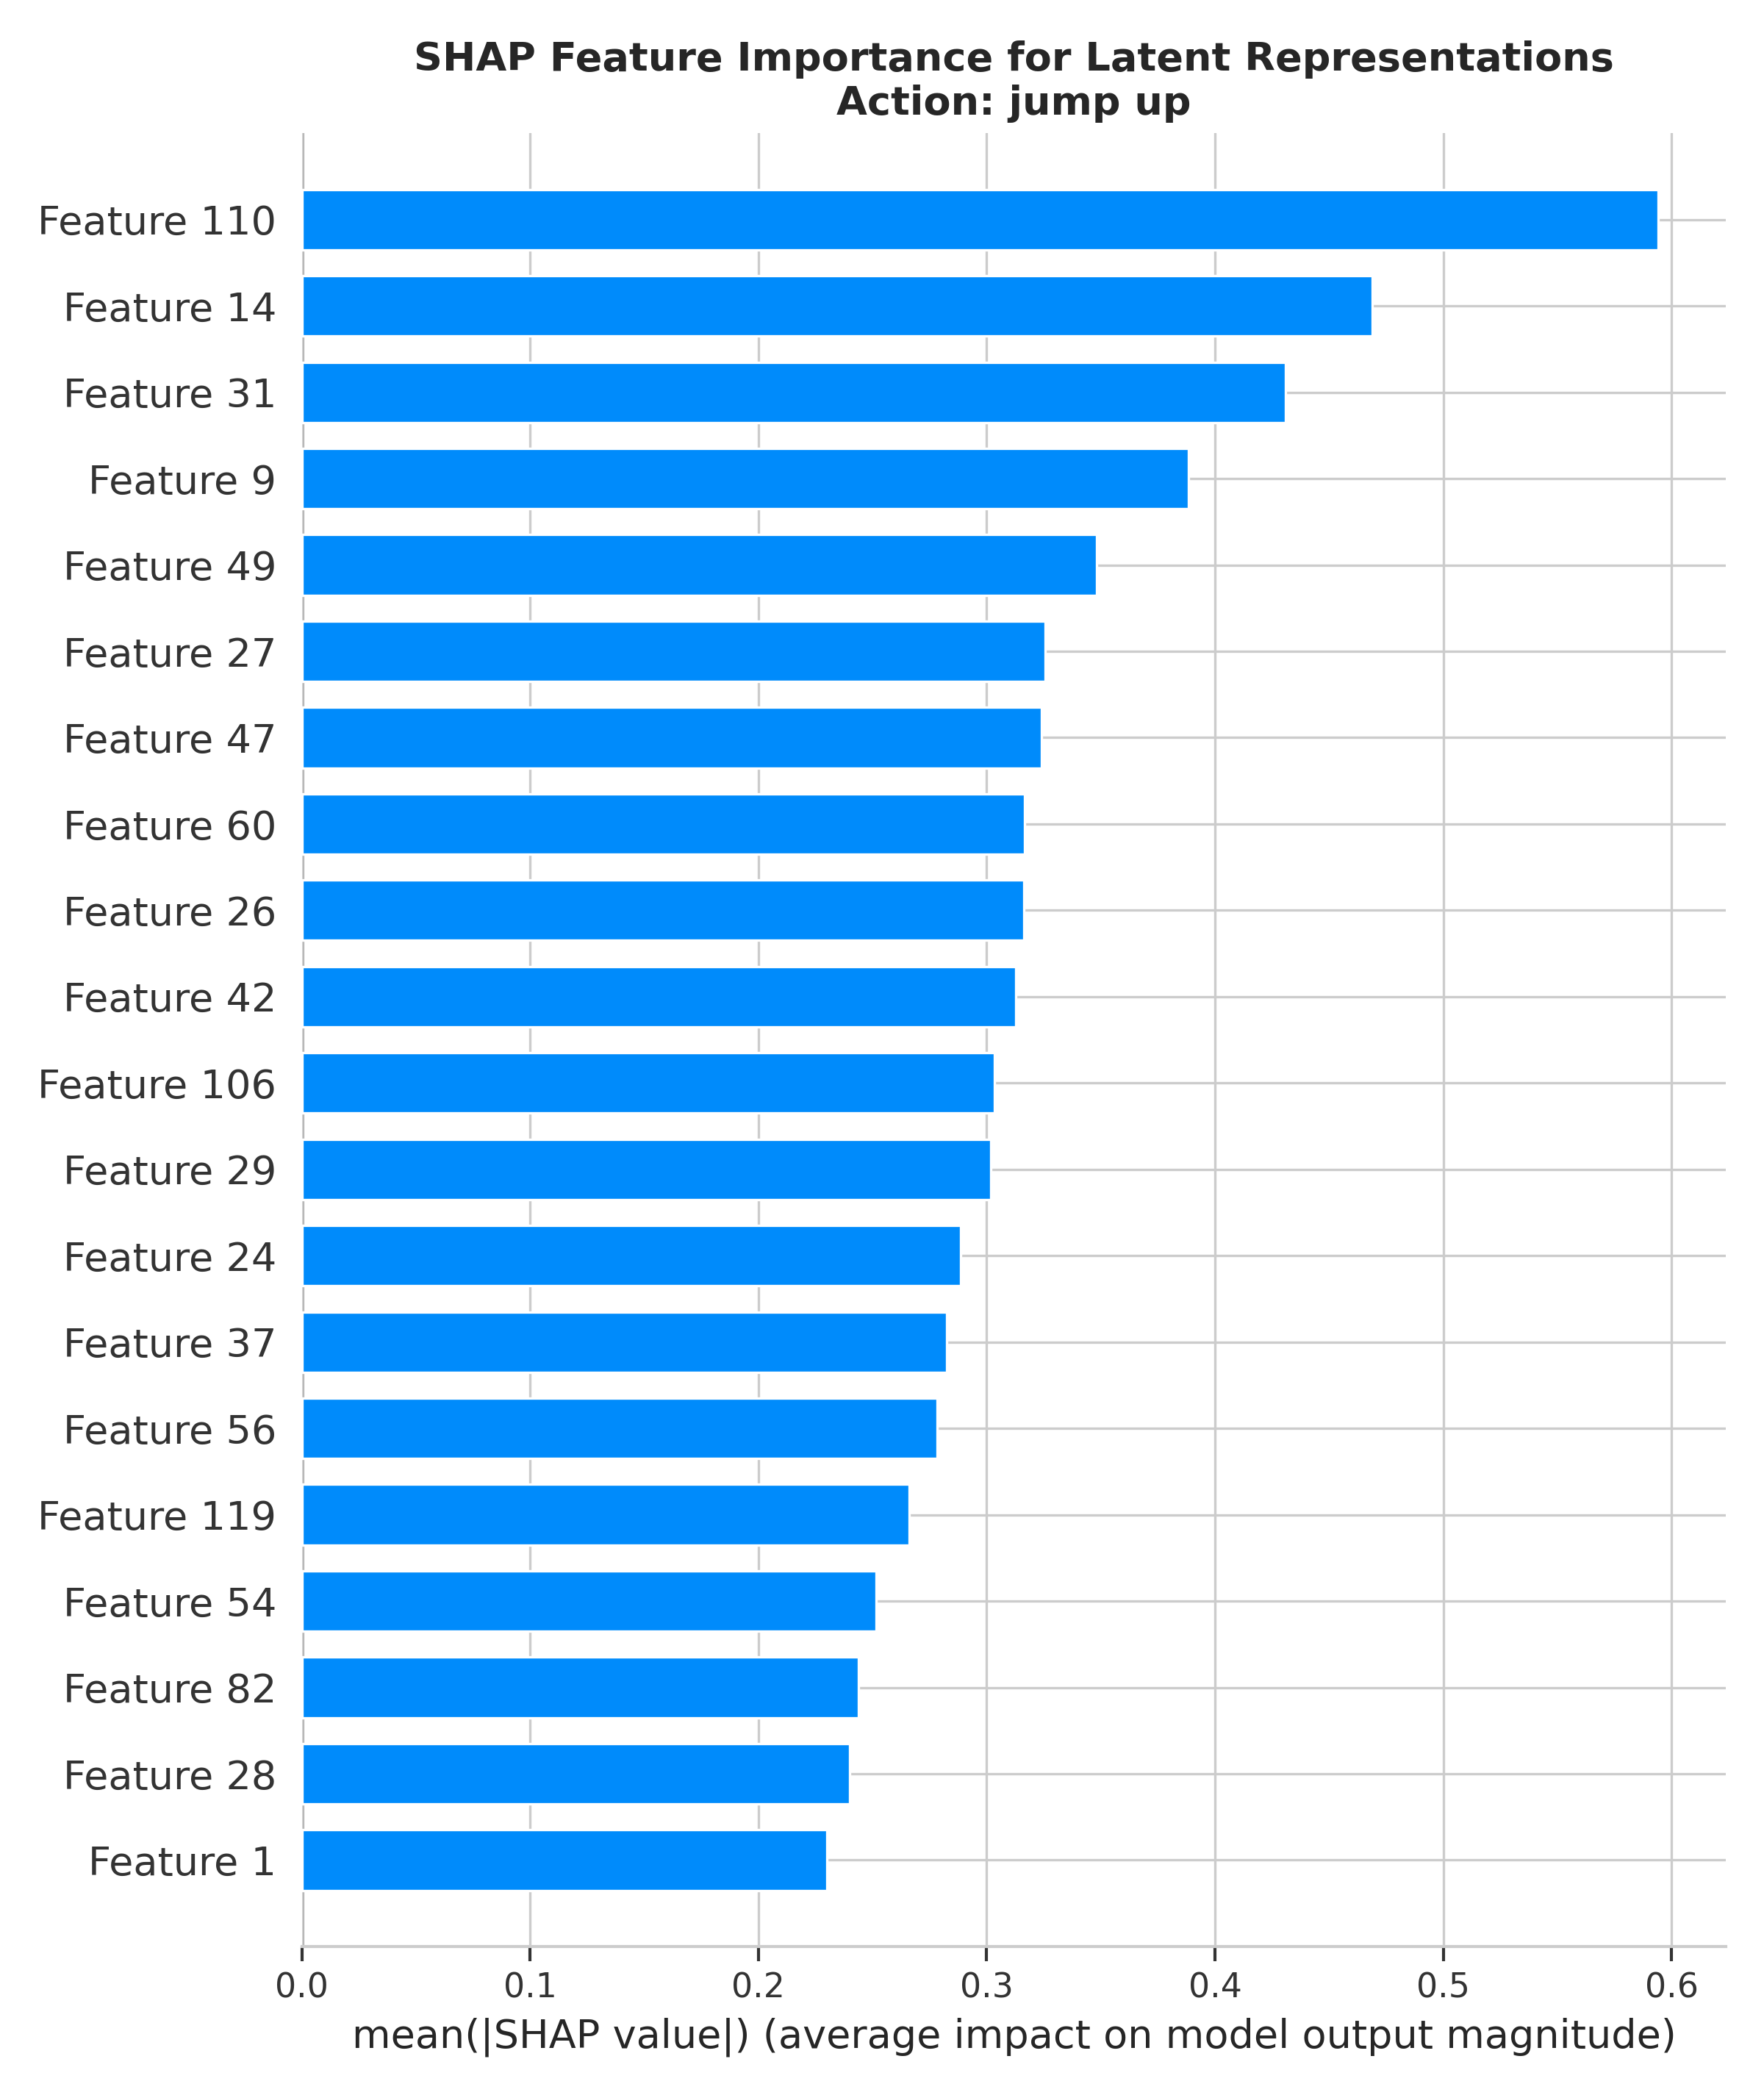
\includegraphics[width=\linewidth]{plots/shap_summary_jumping.png}
        \caption{Đóng góp đặc trưng cho Jumping}
        \label{fig:shap_jumping}
    \end{subfigure}
    \caption{Biểu đồ SHAP Feature Importance giải thích đóng góp của các đặc trưng ẩn S-JEPA vào quyết định phân lớp.}
    \label{fig:shap_comparison}
\end{figure*}
Chúng tôi áp dụng kỹ thuật Gradient Saliency để đánh giá trực tiếp mức độ nhạy cảm của dự đoán đầu ra đối với các khớp xương. Phương pháp này là nền tảng toán học của các giải thuật CAM, Grad-CAM, Grad-CAM++ và Integrated Gradients. Độ nhạy $S_{t, j}$ của khớp $j$ tại khung hình $t$ đối với lớp hành động $c$ được tính bằng chuẩn L2 của gradient của điểm số dự đoán $f_c(\mathbf{X})$ theo tọa độ khớp $\mathbf{p}_{t}^j$:
\begin{equation}
S_{t, j} = \left\| \nabla_{\mathbf{p}_{t}^j} f_c(\mathbf{X}) \right\|_2
\end{equation}
Các giá trị này được chuẩn hóa về đoạn $[0, 1]$ để vẽ bản đồ nhiệt (Hình \ref{fig:saliency_comparison}):
\begin{itemize}
    \item \textbf{Hành động Vẫy tay (Hình \ref{fig:saliency_heatmap_waving}):} Độ nhạy tập trung cao độ vào khớp bàn tay trái/phải (khớp 7 và 11) trong các khung hình thực hiện động tác vẫy.
    \item \textbf{Hành động Nhảy (Hình \ref{fig:saliency_heatmap_jumping}):} Độ nhạy tập trung mạnh vào khớp đầu (khớp 3) và các khớp chi dưới (khớp gối, cổ chân 15 và 19) tại các khung hình cất đất và tiếp đất.
\end{itemize}
Kết quả này khẳng định mô hình thực sự dựa vào động học hình học của đúng các bộ phận khớp chuyển động đặc trưng để đưa ra quyết định phân loại, tương tự như cơ chế định vị vùng đặc trưng của Grad-CAM.



\subsection{Giải thích đặc trưng ẩn bằng Giá trị Shapley (XAI - SHAP)}

\begin{figure*}[t]
\centering
\resizebox{0.95\textwidth}{!}{%
\begin{tikzpicture}[
    node distance=0.8cm and 1.2cm,
    block/.style={draw, rectangle, fill=blue!10, text width=2.2cm, minimum height=0.8cm, align=center, rounded corners, font=\small},
    input/.style={draw, ellipse, fill=gray!10, text width=1.8cm, minimum height=0.6cm, align=center, font=\small},
    classifier/.style={draw, rectangle, fill=green!10, text width=2.2cm, minimum height=0.8cm, align=center, rounded corners, font=\small},
    fusion/.style={draw, circle, fill=yellow!15, minimum size=1.2cm, align=center, font=\small},
    output/.style={draw, rectangle, fill=red!10, text width=2.2cm, minimum height=0.6cm, align=center, rounded corners, font=\small},
    arrow/.style={-latex, thick}
]

    % Inputs
    \node [input] (in_joint) {Joint Sequence};
    \node [input, below=of in_joint, yshift=-0.2cm] (in_bone) {Bone Sequence};
    \node [input, below=of in_bone, yshift=-0.2cm] (in_velo) {Velocity Sequence};

    % Encoders
    \node [block, right=of in_joint] (enc_joint) {S-JEPA Encoder\\(Joint)};
    \node [block, right=of in_bone] (enc_bone) {S-JEPA Encoder\\(Bone)};
    \node [block, right=of in_velo] (enc_velo) {S-JEPA Encoder\\(Velocity)};

    % Linear Classifiers
    \node [classifier, right=of enc_joint] (cls_joint) {Linear Probing\\Classifier};
    \node [classifier, right=of enc_bone] (cls_bone) {Linear Probing\\Classifier};
    \node [classifier, right=of enc_velo] (cls_velo) {Linear Probing\\Classifier};

    % Fusion Node
    \node [fusion, right=of cls_bone, xshift=0.5cm] (fusion) {Weighted\\Late\\Fusion};

    % Output
    \node [output, right=of fusion] (out) {Predicted\\Action Class};

    % Connections
    \draw [arrow] (in_joint) -- (enc_joint);
    \draw [arrow] (in_bone) -- (enc_bone);
    \draw [arrow] (in_velo) -- (enc_velo);

    \draw [arrow] (enc_joint) -- (cls_joint);
    \draw [arrow] (enc_bone) -- (cls_bone);
    \draw [arrow] (enc_velo) -- (cls_velo);

    \draw [arrow] (cls_joint) -| node[above, xshift=-0.5cm, font=\scriptsize] {$\alpha \cdot P_J$} (fusion);
    \draw [arrow] (cls_bone) -- node[above, font=\scriptsize] {$\beta \cdot P_B$} (fusion);
    \draw [arrow] (cls_velo) -| node[below, xshift=-0.5cm, font=\scriptsize] {$\gamma \cdot P_V$} (fusion);

    \draw [arrow] (fusion) -- (out);

\end{tikzpicture}%
}
\caption{Sơ đồ quy trình phân lớp đa luồng kết hợp muộn (Multi-stream Late Fusion pipeline) của mô hình S-JEPA.}
\label{fig:late_fusion_arch}
\end{figure*}
Để giải thích hậu nghiệm (post-hoc) cơ chế đóng góp của các đặc trưng ẩn (latent features) của mô hình S-JEPA vào bộ phân lớp tuyến tính downstream, chúng tôi áp dụng lý thuyết trò chơi hợp tác SHAP (Shapley Additive exPlanations). Đây là phương pháp độc lập mô hình (Model-Agnostic) tương tự LIME và ANCHORS. Giá trị Shapley $\phi_i$ đo lường đóng góp biên của đặc trưng thứ $i$ trong tập đặc trưng không gian ẩn $F$ vào kết quả dự đoán của bộ phân lớp:
\begin{equation}
\label{eq:shap_val}
\phi_i = \sum_{S \subseteq F \setminus \{i\}} \frac{|S|!(|F| - |S| - 1)!}{|F|!} [v(S \cup \{i\}) - v(S)]
\end{equation}
Trong đó $S$ là tập con các đặc trưng được chọn từ không gian ẩn không chứa đặc trưng $i$, và $v(S)$ là kỳ vọng có điều kiện của điểm dự đoán lớp hành động khi biết các đặc trưng trong $S$.

Biểu đồ SHAP Feature Importance (Hình \ref{fig:shap_comparison}) thể hiện đóng góp biên của các chiều ẩn. Phân tích chỉ ra chỉ một nhóm nhỏ khoảng 10 đặc trưng ẩn là có đóng góp biên vượt trội cho mỗi lớp hành động. Các đặc trưng mang thông tin về chuyển động tay đóng góp tích cực cho lớp Waving Hand, trong khi các đặc trưng mô tả biến thiên độ cao đóng góp tích cực cho lớp Jumping. Điều này giúp giải thích toán học tính minh bạch của không gian latent S-JEPA.



\subsection{Đánh giá Mô hình Downstream và Phân tích Lỗi}

\begin{figure}[htbp]
    \centering
    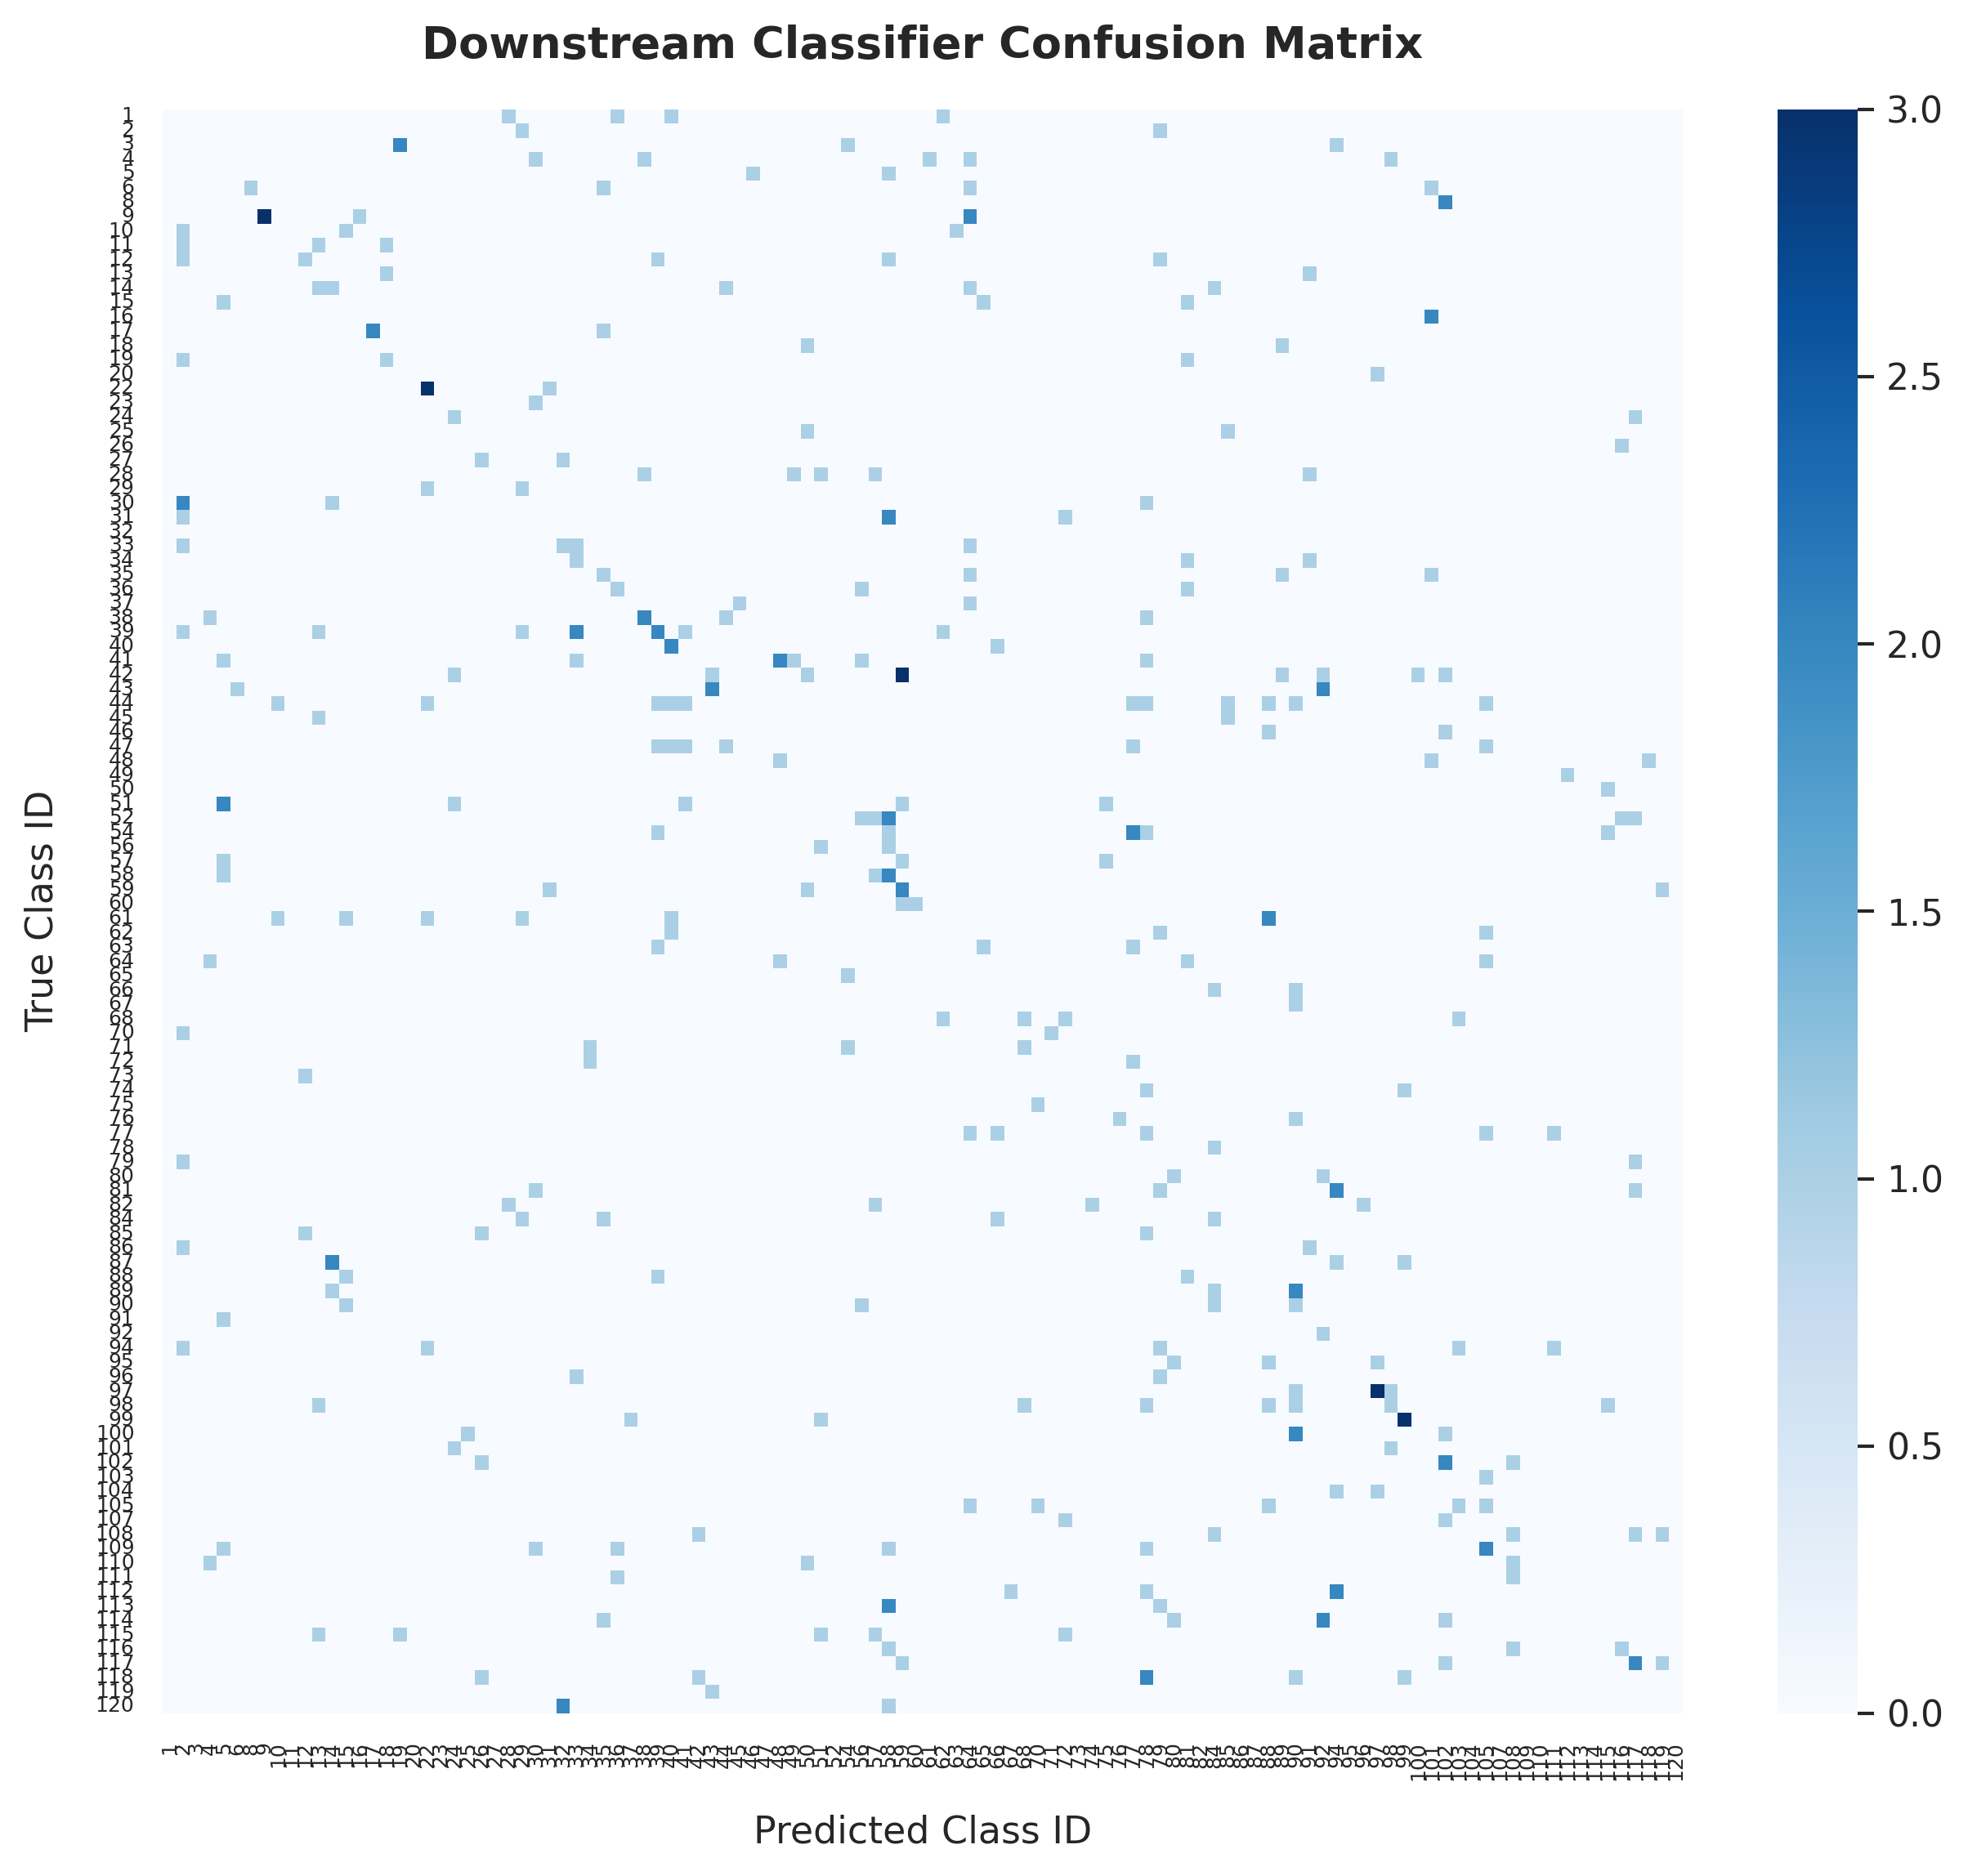
\includegraphics[width=\linewidth]{plots/confusion_matrix.png}
    \caption{Ma trận nhầm lẫn (Confusion Matrix Heatmap) của mô hình phân lớp downstream.}
    \label{fig:confusion_matrix}
\end{figure}
Để đánh giá định lượng năng lực biểu diễn của S-JEPA, chúng tôi tiến hành đánh giá độ chính xác phân loại thông qua mô hình phân lớp tuyến tính (Linear Probing) trên ba luồng đặc trưng đơn lẻ (Joint, Bone, Velocity) và kết hợp Ensemble thông qua kỹ thuật Weighted Late Fusion (sơ đồ quy trình được chi tiết trong Hình \ref{fig:late_fusion_arch}).


 

Kết quả thực nghiệm được tổng hợp trong Bảng \ref{tab:results}:
- \textbf{Luồng đơn lẻ:} Luồng khớp xương (Joint) đạt kết quả tốt nhất với $89.52\%$ trên NTU-60 X-View và $73.73\%$ trên NTU-120 X-Sub. Luồng xương nối (Bone) cho kết quả bám đuổi sát sao, trong khi luồng vận tốc (Velocity) đạt mức thấp hơn nhưng mang thông tin bổ trợ động lực học quan trọng.
- \textbf{Ensemble Late Fusion:} Bằng cách tìm kiếm lưới (Grid Search) bộ trọng số tối ưu (NTU-60: $\alpha=0.8, \beta=1.0, \gamma=0.9$; NTU-120: $\alpha=1.1, \beta=1.3, \gamma=1.7$), việc kết hợp ba luồng giúp nâng độ chính xác đáng kể lên \textbf{92.94\%} (NTU-60) và \textbf{78.30\%} (NTU-120). Điều này khẳng định tính bổ trợ thông tin lẫn nhau của các luồng đặc trưng hình học.

\begin{table*}[t]
\begin{minipage}[t]{0.48\textwidth}
\centering
\caption{Độ chính xác phân loại hành động của S-JEPA trên các luồng dữ liệu đơn và tổ hợp Ensemble Late Fusion.}
\label{tab:results}
\resizebox{\linewidth}{!}{%
\begin{tabular}{lcc}
\toprule
\textbf{Phương pháp / Luồng dữ liệu} & \textbf{NTU-60 X-View (\%)} & \textbf{NTU-120 X-Sub (\%)} \\
\midrule
Luồng Khớp xương (Joint Stream) & 89.52 & 73.73 \\
Luồng Xương nối (Bone Stream) & 88.80 & 71.72 \\
Luồng Vận tốc (Velocity Stream) & 84.70 & 65.81 \\
\midrule
\textbf{Ensemble Late Fusion} & \textbf{92.94} & \textbf{78.30} \\
\bottomrule
\end{tabular}%
}
\end{minipage}
\hfill
\begin{minipage}[t]{0.48\textwidth}
\centering
\caption{So sánh độ chính xác Acc@1 (\%) của S-JEPA (Multi-stream Late Fusion) với các phương pháp học tự giám sát SOTA khác.}
\label{tab:sota_comparison}
\resizebox{\linewidth}{!}{%
\begin{tabular}{llcc}
\toprule
\textbf{Phương pháp} & \textbf{Đầu vào} & \textbf{NTU-60 X-View} & \textbf{NTU-120 X-Sub} \\
\midrule
LongTGAN \cite{b4} & Joint & 48.1 & - \\
SkeletonMAE \cite{b4} & Joint & 77.7 & 72.5 \\
CrossCLR \cite{b5} & Joint+Bone+Motion & 83.4 & 67.9 \\
AimCLR \cite{b5} & Joint+Bone+Motion & 83.8 & 68.2 \\
ActCLR \cite{b6} & Joint+Bone+Motion & 88.8 & 74.3 \\
MAMP \cite{b3} & Joint & 89.1 & \textbf{78.6} \\
\midrule
\textbf{S-JEPA (Ours - Joint)} & Joint & 89.52 & 73.73 \\
\textbf{S-JEPA (Ours - Ensemble)} & Joint+Bone+Velo & \textbf{92.94} & \textbf{78.30} \\
\bottomrule
\end{tabular}%
}
\end{minipage}
\end{table*}

Bên cạnh đó, để đặt kết quả thực nghiệm trong hệ quy chiếu với các công trình nghiên cứu hiện đại khác, chúng tôi so sánh hiệu năng phân loại của S-JEPA (Joint và Ensemble) với các mô hình học tự giám sát khác trên tập dữ liệu NTU-60 (X-View) và NTU-120 (X-Sub) ở Bảng \ref{tab:sota_comparison}:
\begin{itemize}
    \item Các phương pháp học đối sánh (như ActCLR \cite{b6}) và che phủ sinh (như MAMP \cite{b3}) đạt kết quả tương đối cao nhờ áp dụng tăng cường dữ liệu phức tạp hoặc học tái dựng chuyển động.
    \item S-JEPA (Joint chỉ dùng khớp xương) đạt kết quả cạnh tranh trực tiếp ($89.52\%$ trên NTU-60 và $73.73\%$ trên NTU-120). Khi kết hợp đa luồng qua Ensemble Late Fusion, mô hình của chúng tôi vượt qua hầu hết các mô hình học tự giám sát khác, đạt hiệu năng phân lớp tuyến tính vô cùng xuất sắc với \textbf{92.94\%} (NTU-60) và \textbf{78.30\%} (NTU-120), tiệm cận mức tối ưu của các phương pháp tự giám sát phức tạp hơn.
\end{itemize}

Ma trận nhầm lẫn dạng Heatmap (Hình \ref{fig:confusion_matrix}) cung cấp góc nhìn sâu sắc về hiệu năng phân loại của mô hình phân lớp downstream:
\begin{itemize}
    \item Các hành động di chuyển chân (như Đi bộ - Walking) có độ chính xác rất cao nhờ đặc trưng vận tốc khớp gối đặc thù.
    \item Xảy ra sự nhầm lẫn nhẹ giữa các cặp tương tác gần nhau như Đấm (Punching) và Đẩy (Pushing) do sự tương đồng lớn ở chuyển động vươn vai và duỗi thẳng khớp khuỷu tay.
\end{itemize}




\clearpage
\section{Kết luận}
Nghiên cứu này đã triển khai và thực nghiệm thành công hệ thống học tự giám sát S-JEPA cho bài toán nhận dạng hành động dựa trên khung xương 3D NTU RGB+D 120, gắn liền với các kiến thức cốt lõi trong quy trình khoa học dữ liệu. Bằng cách kết hợp các công cụ phân tích động học khớp xương (EDA), các phương pháp tiền xử lý và loại bỏ điểm ngoại lai thống kê, phân tích tương quan đặc trưng tuyến tính/phi tuyến (Pearson, Spearman, Chi-square), giảm chiều trích xuất tính năng hình học (PCA, Kernel PCA, ISOMAP, LDA) và giải thích mô hình thông qua XAI (SHAP, Attention, Gradient Saliency), chúng tôi đã hoàn thiện một hệ thống phân tích và trực quan hóa dữ liệu toàn diện, mở ra hướng đi đầy hứa hẹn cho các ứng dụng giám sát hành vi người trong thực tế.

\section*{Tài liệu tham khảo}
\begin{thebibliography}{00}
\bibitem{b1} Shahroudy, A., Liu, J., Ng, T. T., \& Wang, G. (2016). Ntu rgb+ d: A large scale dataset for 3d human activity analysis. In \textit{Proceedings of the IEEE conference on computer vision and pattern recognition} (pp. 1010-1019).
\bibitem{b2} Assran, M., Caron, M., Misra, I., Bojanowski, P., Joulin, A., Nicolas, M., ... \& LeCun, Y. (2023). Self-supervised learning from images with a joint-embedding predictive architecture. In \textit{Proceedings of the IEEE/CVF Conference on Computer Vision and Pattern Recognition} (pp. 15619-15629).
\bibitem{b3} Feichtenhofer, C., Li, Y., \& He, K. (2022). Masked autoencoders are spatiotemporal learners. In \textit{Proceedings of the IEEE/CVF Conference on Computer Vision and Pattern Recognition} (pp. 12593-12602).
\bibitem{b4} Yan, H., Liu, Y., Wei, Y., Li, Z., Li, G., \& Lin, L. (2023). Skeletonmae: graph-based masked autoencoder for skeleton sequence pre-training. In \textit{Proceedings of the IEEE/CVF International Conference on Computer Vision} (pp. 5606-5618).
\bibitem{b5} Guo, T., Liu, H., Chen, Z., Liu, M., Wang, T., \& Ding, R. (2022). Contrastive learning from extremely augmented skeleton sequences for self-supervised action recognition. In \textit{Proceedings of the AAAI Conference on Artificial Intelligence} (pp. 762-770).
\bibitem{b6} Lin, L., Zhang, J., \& Liu, J. (2023). Actionlet-dependent contrastive learning for unsupervised skeleton-based action recognition. In \textit{Proceedings of the IEEE/CVF Conference on Computer Vision and Pattern Recognition} (pp. 14454-14463).
\bibitem{b7} Abdelfattah, M. \& Alahi, A. (2024). S-jepa: A joint embedding predictive architecture for skeletal action recognition. In \textit{Proceedings of the IEEE/CVF Conference on Computer Vision and Pattern Recognition} (pp. 1112-1121).
\bibitem{b8} Abnar, S. \& Zuidema, W. (2020). Quantifying attention flow in transformers. In \textit{Proceedings of the 58th Annual Meeting of the Association for Computational Linguistics} (pp. 4190-4197).
\bibitem{b9} Simonyan, K., Vedaldi, A., \& Zisserman, A. (2013). Deep inside convolutional networks: Visualising image classification models and saliency maps. \textit{arXiv preprint arXiv:1312.6034}.
\bibitem{b10} Lundberg, S. M. \& Lee, S.-I. (2017). A unified approach to interpreting model predictions. In \textit{Advances in neural information processing systems} (pp. 4765-4774).
\end{thebibliography}

\end{document}
